\documentclass[a4paper]{article}
\usepackage{cmap}
\usepackage[utf8]{inputenc}
\usepackage[T2A]{fontenc}
\usepackage[english,russian]{babel} 
\usepackage[left=15mm, top=15mm, right=15mm, bottom=42mm, nohead, nofoot]{geometry}
\usepackage{blindtext}  % рыба-текст
\usepackage{graphicx}  % изобржаения
\usepackage{float} % плавающие объекты
\usepackage{wrapfig}  % изобржаения
\usepackage{tikz} % графика
\usepackage{xcolor} % определение цветов
\usepackage{nicefrac} % красивые дроби
\usepackage{cancel} % сокращение
\usepackage{amsmath,amsfonts,amssymb} % математический пакет
\usepackage{hyperref}  % гиперссылки
\usepackage{fancybox,fancyhdr} % хедер и футер
\usepackage{listings} % код
\usepackage{accsupp}
\pagestyle{fancy}
\fancyhf{}
\fancyhead[L]{Лабораторная работа №6}
\fancyhead[R]{\textit{Обработка изображений}}
\fancyfoot[C]{\thepage}
\headsep=8mm
\footskip=20mm

\definecolor{urlcolor}{HTML}{3454D1}
\definecolor{linkcolor}{HTML}{3454D1}
\hypersetup{pdfstartview=FitH, linkcolor=linkcolor, urlcolor=urlcolor, colorlinks=true}

\definecolor{strings}{rgb}{0,0.6,0}
\definecolor{comments}{rgb}{0,0.3,0}
\definecolor{numbers}{rgb}{0.5,0.5,0.5}
\definecolor{keywords}{rgb}{0.09,0.61,0.95}
\definecolor{background}{rgb}{0.97,0.97,0.97}
\newcommand{\noncopynumber}[1]{%
    \BeginAccSupp{method=escape,ActualText={}}%
    #1%
    \EndAccSupp{}%
}
\lstdefinestyle{codestyle}{
    backgroundcolor=\color{background},
    commentstyle=\color{comments},
    keywordstyle=\color{keywords},
    stringstyle=\color{strings},
    numberstyle=\tiny\color{numbers}\noncopynumber,
    basicstyle=\ttfamily\footnotesize,
    breakatwhitespace=false,
    breaklines=true,
    captionpos=b,
    inputencoding=utf8,
    keepspaces=true,
    numbers=left,
    numbersep=5pt,
    showspaces=false,
    showstringspaces=false,
    showtabs=false,
    tabsize=2,
    extendedchars=true,
    literate=
    {а}{{\cyra}}1
    {б}{{\cyrb}}1
    {в}{{\cyrv}}1
    {г}{{\cyrg}}1
    {д}{{\cyrd}}1
    {е}{{\cyre}}1
    {ж}{{\cyrzh}}1
    {з}{{\cyrz}}1
    {и}{{\cyri}}1
    {й}{{\cyrishrt}}1
    {к}{{\cyrk}}1
    {л}{{\cyrl}}1
    {м}{{\cyrm}}1
    {н}{{\cyrn}}1
    {о}{{\cyro}}1
    {п}{{\cyrp}}1
    {р}{{\cyrr}}1
    {с}{{\cyrs}}1
    {т}{{\cyrt}}1
    {у}{{\cyru}}1
    {ф}{{\cyrf}}1
    {х}{{\cyrh}}1
    {ц}{{\cyrc}}1
    {ч}{{\cyrch}}1
    {ш}{{\cyrsh}}1
    {щ}{{\cyrshch}}1
    {ъ}{{\cyrhrdsn}}1
    {ы}{{\cyrery}}1
    {ь}{{\cyrsftsn}}1
    {э}{{\cyrerev}}1
    {ю}{{\cyryu}}1
    {я}{{\cyrya}}1
    {А}{{\CYRA}}1
    {Б}{{\CYRB}}1
    {В}{{\CYRV}}1
    {Г}{{\CYRG}}1
    {Д}{{\CYR96}}1
    {Е}{{\CYRE}}1
    {Ж}{{\CYRZH}}1
    {З}{{\CYRZ}}1
    {И}{{\CYRI}}1
    {Й}{{\CYRISHRT}}1
    {К}{{\CYRK}}1
    {Л}{{\CYRL}}1
    {М}{{\CYRM}}1
    {Н}{{\CYRN}}1
    {О}{{\CYRO}}1
    {П}{{\CYRP}}1
    {Р}{{\CYRR}}1
    {С}{{\CYRS}}1
    {Т}{{\CYRT}}1
    {У}{{\CYRU}}1
    {Ф}{{\CYRF}}1
    {Х}{{\CYRH}}1
    {Ц}{{\CYRC}}1
    {Ч}{{\CYRCH}}1
    {Ш}{{\CYRSH}}1
    {Щ}{{\CYRSHCH}}1
    {Ъ}{{\CYRHRDSN}}1
    {Ы}{{\CYRERY}}1
    {Ь}{{\CYRSFTSN}}1
    {Э}{{\CYREREV}}1
    {Ю}{{\CYRYU}}1
    {Я}{{\CYRYA}}1
}

\lstset{style=codestyle}

\addto\captionsrussian{
  \renewcommand{\contentsname}
    {\centering Содержание}
}


\newlength{\tempheight}
\newcommand{\Let}{
\mathbin{\text{\settoheight{\tempheight}{\mathstrut}\raisebox{0.4\pgflinewidth}{
\tikz[baseline=0.5ex,line cap=round,line join=round] \draw (0,0) --++ (0.3em,0) --++ (0,2.3ex) --++ (-0.3em,0);
}}}}
\newcommand*\squared[1]{\tikz[baseline=(char.base)]{
            \node[shape=rectangle,draw,inner sep=4pt] (char) {#1};}}
\newcommand*\msquared[1]{\tikz[baseline=(char.base)]{
            \node[shape=rectangle,draw,inner sep=4pt] (char) {$\displaystyle #1$};}}
\newcommand{\at}{\biggr\rvert}
\newcommand{\shiftright}[3]{\makebox[#2][r]{\makebox[#1][l]{#3}}}
\newcommand{\e}{\;\text{e}}
\let\oldint\int
\def\int{\oldint\limits}
\DeclareRobustCommand{\divby}{%
  \mathrel{\vbox{\baselineskip.65ex\lineskiplimit0pt\hbox{.}\hbox{.}\hbox{.}}}%
}

\newcommand\NB{\textbf{N\kern-0.32em\textcolor{red}{B}}}

\begin{document}

\begin{titlepage}
    \begin{center}
        Федеральное государственное автономное образовательное \\ учреждение высшего образования \\[6pt]
        САНКТ-ПЕТЕРБУРГСКИЙ НАЦИОНАЛЬНЫЙ \\ ИССЛЕДОВАТЕЛЬСКИЙ УНИВЕРСИТЕТ ИТМО \\[16pt]
        Факультет систем управления и робототехники \\[26em]
        Лабораторная работа №6 \\[0.5em]
        \textbf{ОБРАБОТКА ИЗОБРАЖЕНИЙ}
    \end{center}\,\\[10em]
    \begin{flushright}
        Студент: Заводин Е.Ю.\\
        Поток: ЧастМет R23 1.6 \\[0.5em]
        Преподаватели: Перегудин А.А.\\
        Догадин Е.В.
    \end{flushright}\,\\[6em]
    \begin{center}
        {\small Санкт-Петербург \\ 2025}
    \end{center}
\end{titlepage}
\setcounter{page}{2}
\tableofcontents\newpage

\section{Фильтрация изображений с периодичностью.}\

Для выполнения задания я выбрал изображение под номером 3:

\begin{figure}[H]
    \centering
    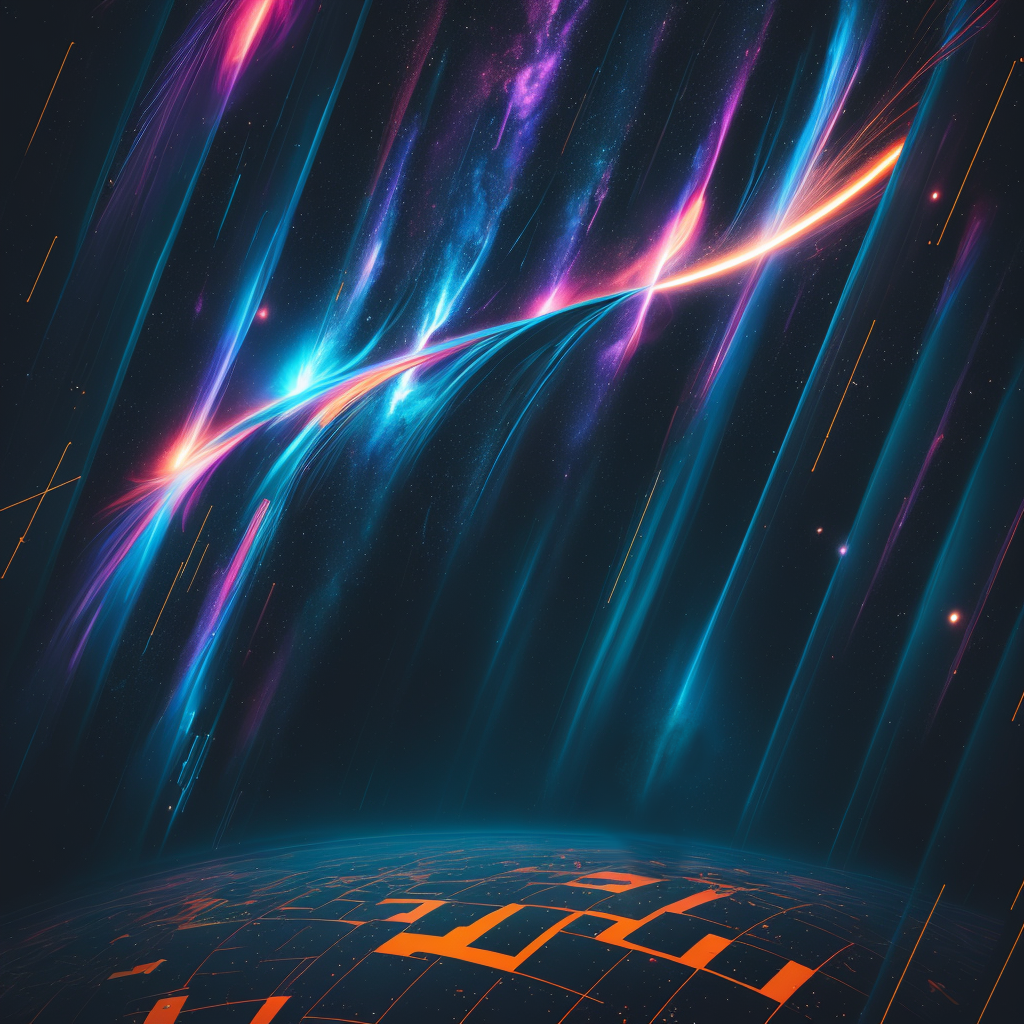
\includegraphics[width=0.51\linewidth]{3.png}
    \caption{Выбранное изображение с периодичностью}
\end{figure}\ 

Его образ Фурье (логарифм модуля образа) получился следующим:

\begin{figure}[H]
    \centering
    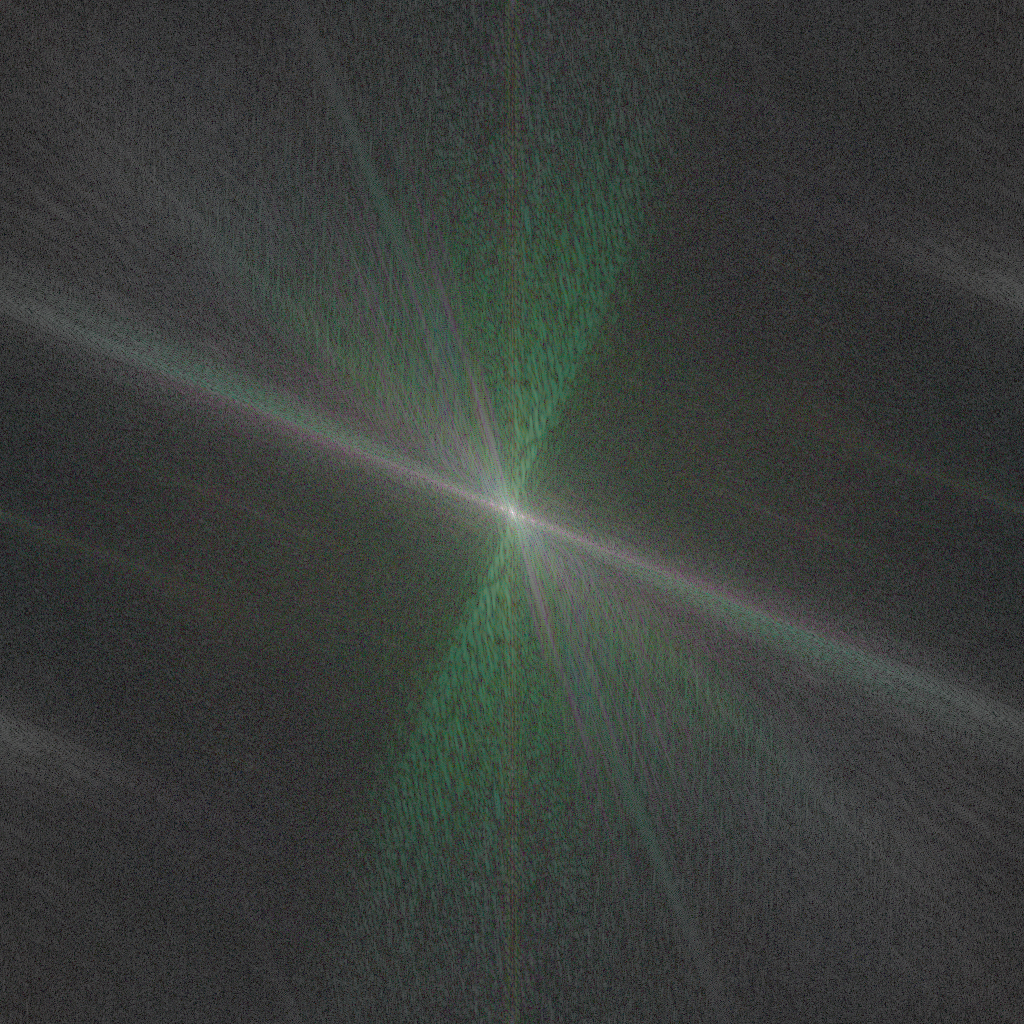
\includegraphics[width=0.51\linewidth]{im3_fourier.png}
    \caption{Изображение логарифма модуля образа исходной картинки}
\end{figure}\

Явные пики, отвечающие за периодичность изображения, находятся в следующих выделенных областях:

\begin{figure}[H]
    \centering
    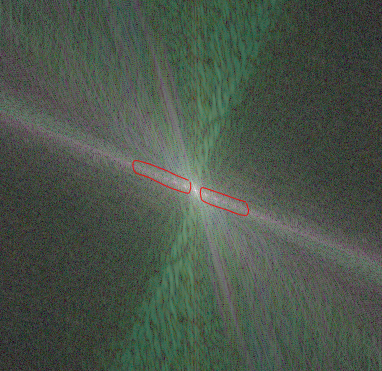
\includegraphics[width=0.51\linewidth]{im3_fourier_highlighted_resized.png}
    \caption{Области, подлежащие редактированию (приближено)}
\end{figure}\

Тогда отфильтрованная картинка будет выглядеть следующим образом:

\begin{figure}[H]
    \centering
    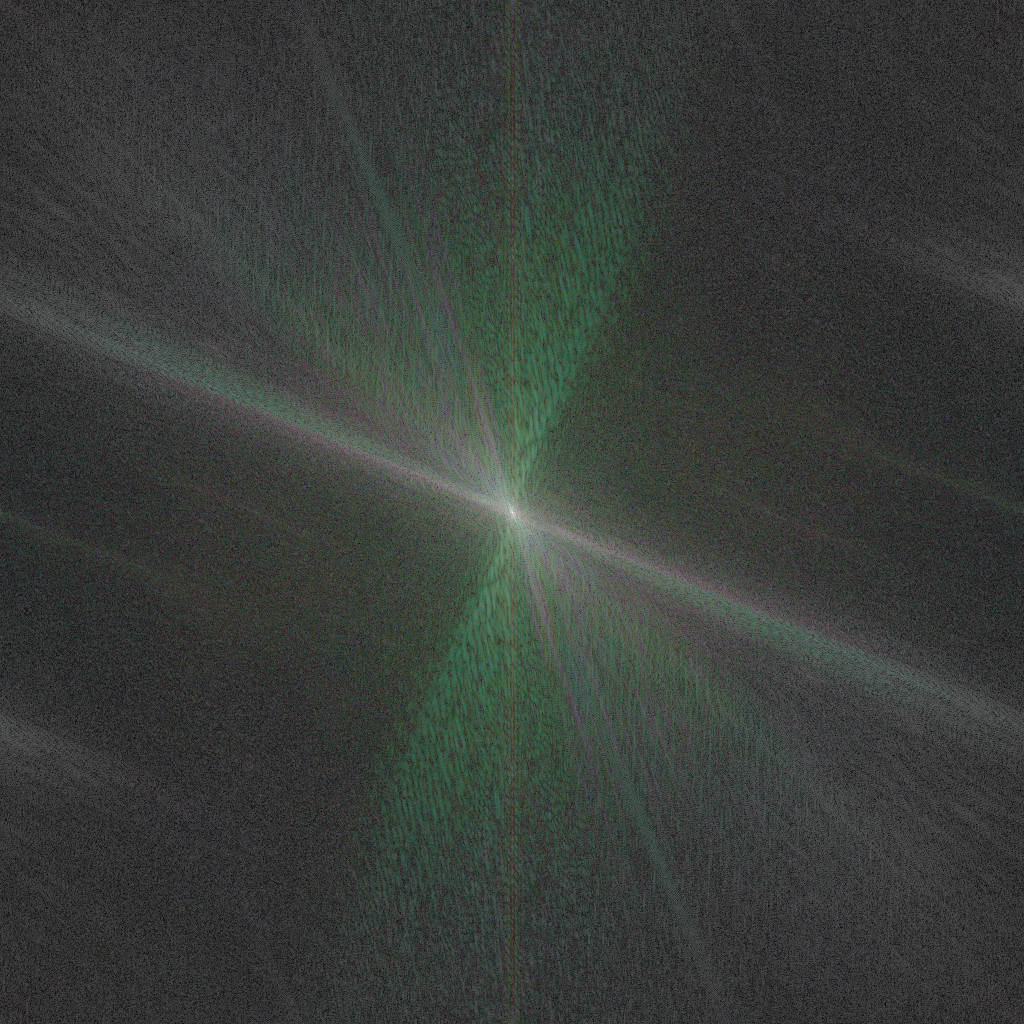
\includegraphics[width=0.51\linewidth]{im3_fourier_recovered.png}
    \caption{Отфильтрованное изображение логарифма модуля образа}
\end{figure}\

Найдем обратное преобразование Фурье при помощи этой картинки в качестве модуля образа, фазу оставим неизменной. Вот результат:

\begin{figure}[H]
    \begin{minipage}{0.49\textwidth}
        \centering 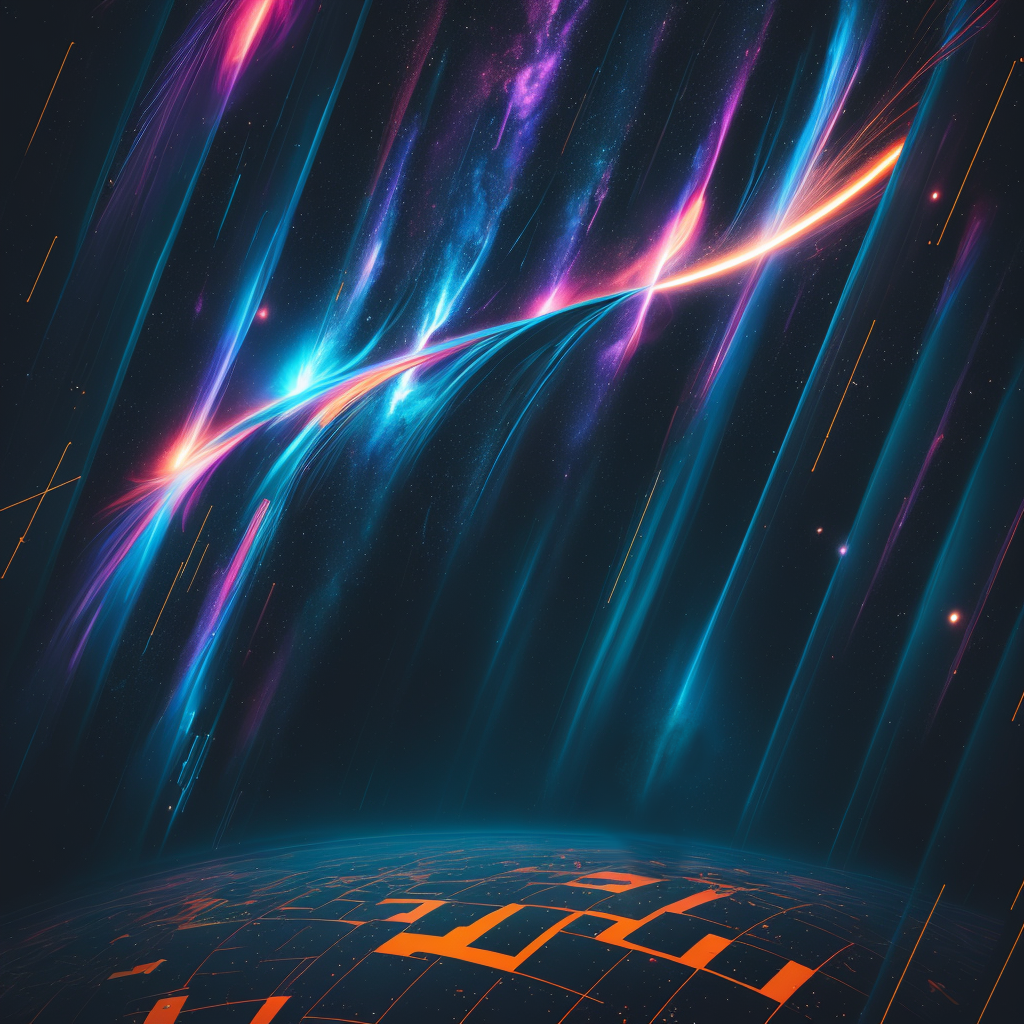
\includegraphics[width=\textwidth]{3.png}
        \caption{Исходное изображение}
    \end{minipage}\hfill
    \begin{minipage}{0.49\textwidth}
        \centering 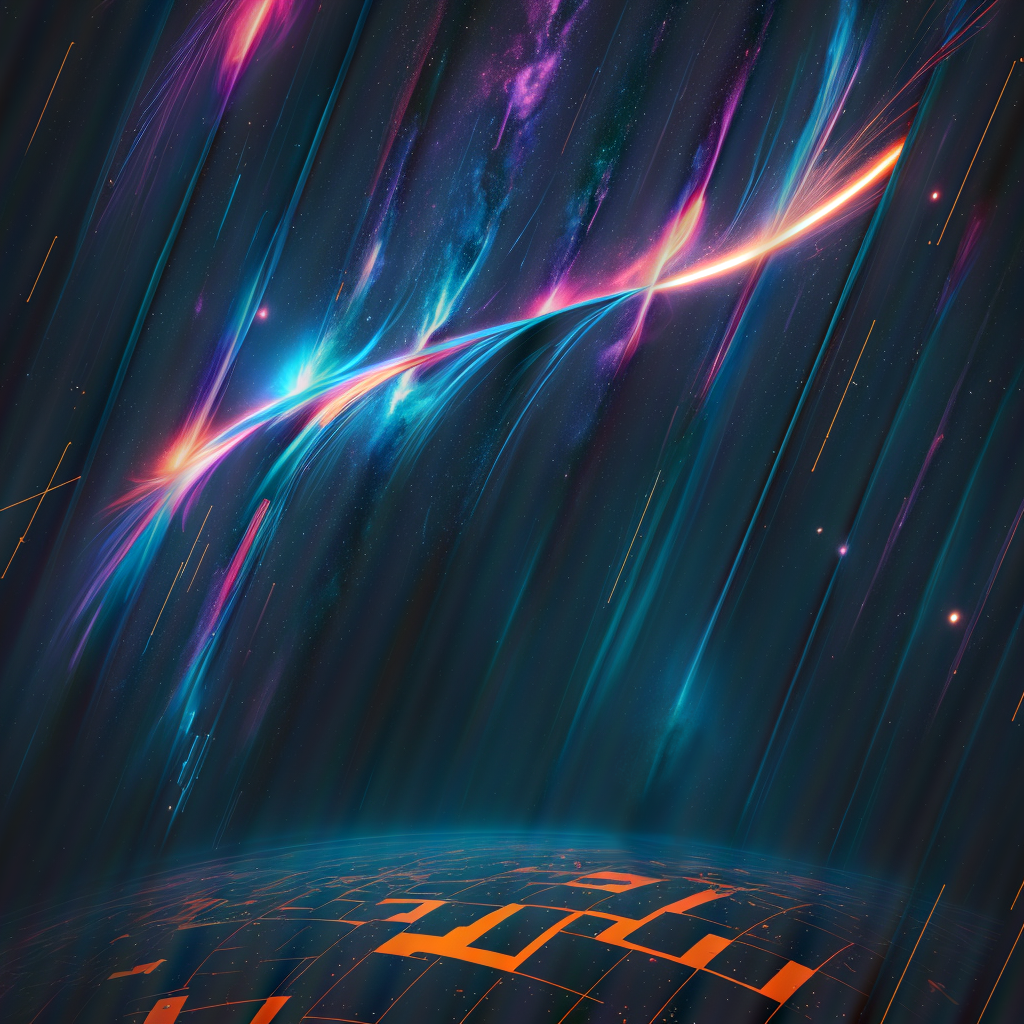
\includegraphics[width=\textwidth]{im3_recovered.png}
        \caption{Фильтрованное изображение}
    \end{minipage}\\[1em]
\end{figure}\noindent\

Также можно заметить на изображении логарифма модуля образа исходной картинки светлые области:

\begin{figure}[H]
    \centering
    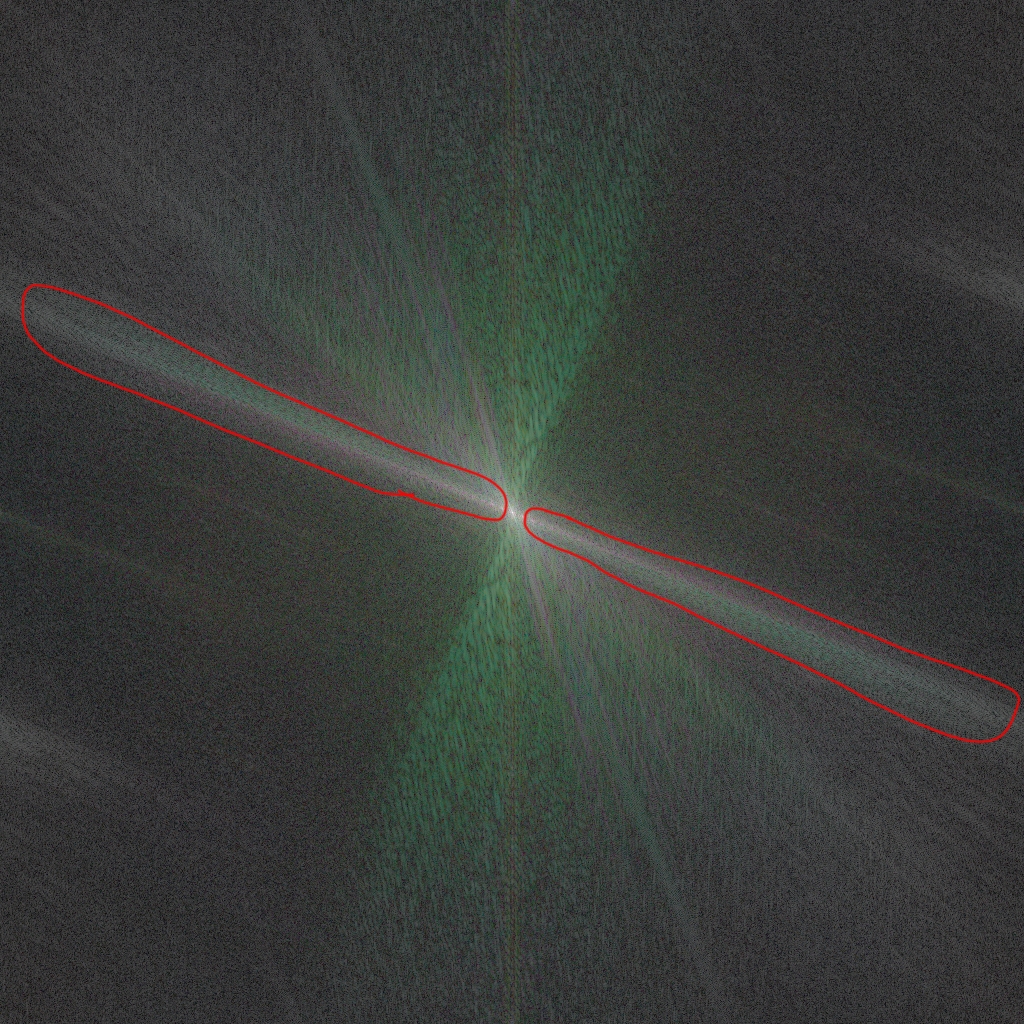
\includegraphics[width=0.51\linewidth]{1/im3_fourier_highlighted.png}
    \caption{Области, которые также можно изменить}
\end{figure}\

Уменьшим амплитуду в этих областях, затемнив соответствующие части изображения:

\begin{figure}[H]
    \begin{minipage}{0.49\textwidth}
        \centering 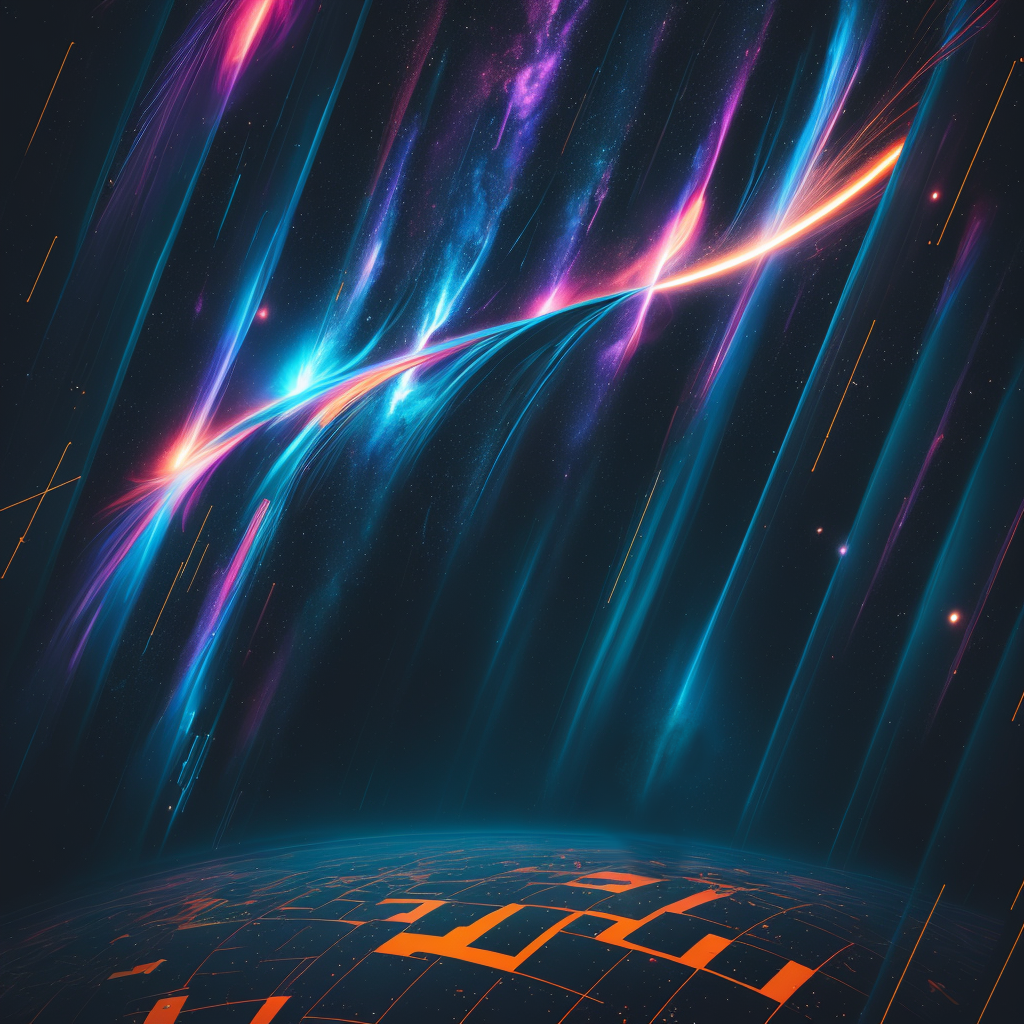
\includegraphics[width=\textwidth]{3.png}
        \caption{Исходное изображение}
    \end{minipage}\hfill
    \begin{minipage}{0.49\textwidth}
        \centering 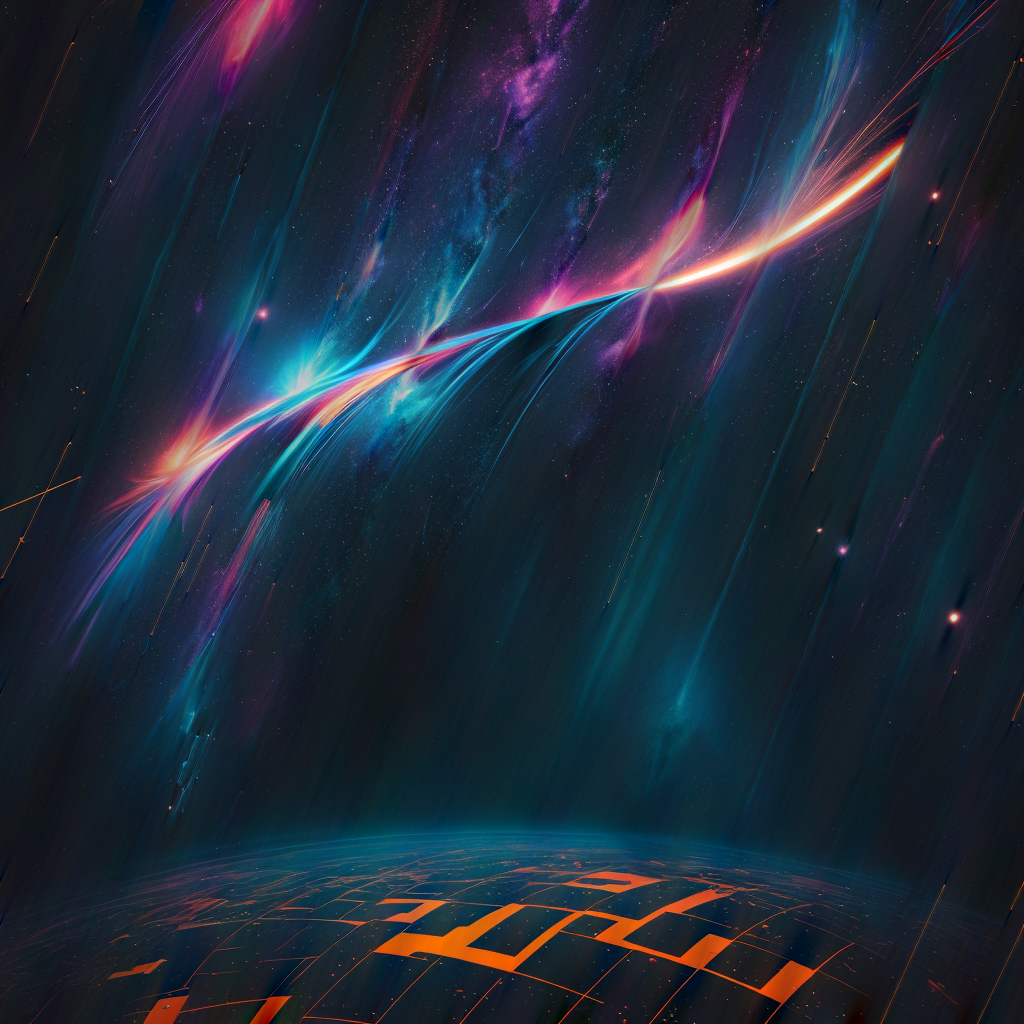
\includegraphics[width=\textwidth]{1/im3_recovered.png}
        \caption{Новое фильтрованное изображение}
    \end{minipage}\\[1em]
\end{figure}\noindent\

Видим, что изображение стало ещё менее периодичным, хоть были обнулены и не только явные пики, как это было на лекции (однако стало заметно тусклее оригинала).

\subsection{Выводы}\ 

Избавиться от периодичности изображения при помощи двумерного преобразования Фурье можно аналогично избавлению от гармонического шума при одномерном преобразовании Фурье -- уменьшив пики на соответствующих частотах образа.

\section{Исследование свертки.}\

Для выполнения этого задания было выбрано следующее изображение размером 480x480 пикселей:

\begin{figure}[H]
    \centering
    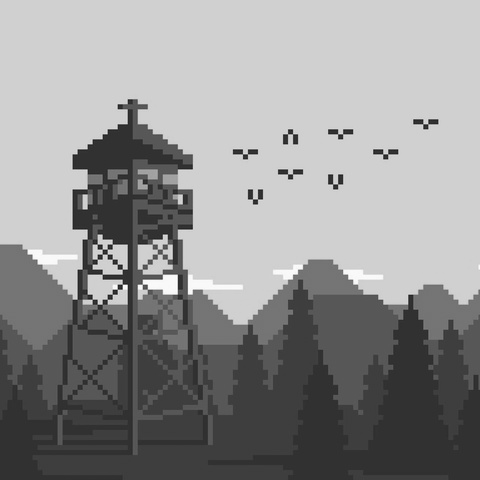
\includegraphics[width=0.51\linewidth]{2/image.png}
    \caption{Исходное черно-белое изображение}
\end{figure}\

Для этой картинки логарифм модуля образа выглядит следующим образом:

\begin{figure}[H]
    \centering
    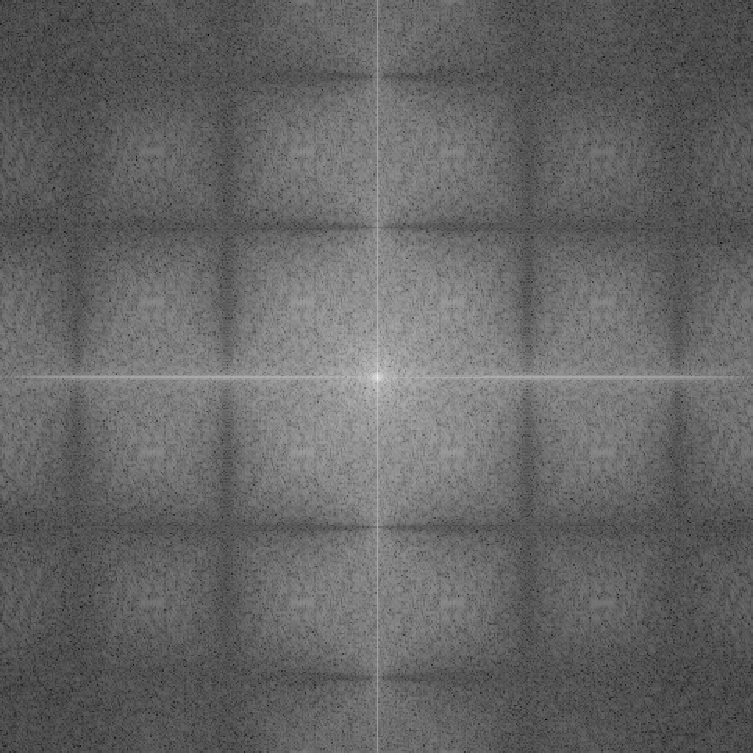
\includegraphics[width=0.51\linewidth]{2/abs_fourier_log_norm_image.png}
    \caption{Изображение логарифма модуля образа исходного изображения}
\end{figure}\

В процессе выполнения задания будем сворачивать исходное изображение с различными ядрами свертки, и сравнивать получившийся результат с аналогичным, полученным через преобразование Фурье из свойства

$$
f * g = \mathcal{F}^{-1}\{\mathcal{F}\{f\}\mathcal{F}\{g\}\}.
$$

В нашем случае $f$ -- исходное изображение, $g$ -- ядро свертки.

\subsection{Ядро размытия по Гауссу}\ 

Строится это ядро следующим образом:

$$
\sigma=\frac{N-1}{6}, A_{ij}=\exp{\left(-\frac{(i-\frac{N+1}{2})^2+(j-\frac{N+1}{2})^2}{2\sigma^2}\right)}, \, i,j \in \{1, \dots, N\}
$$

$$
K_\sigma = \frac{A}{\sum_{i,j}A_{ij}}, \, \text{где $A$ -- вся матрица}
$$\

Свернем его с исходным изображением при разных $N$ и сравним результат с обратным преобразованием Фурье от произведения образов исходного изображения и ядра свертки.\ 

При $N = 3$:


\begin{figure}[H]
    \centering
    
\includegraphics[width=0.51\linewidth]{2/3_abs_fourier_log_norm_gaussian.png}
    \caption{Изображение логарифма модуля образа ядра блочного размытия}\
    
    \begin{minipage}{0.49\textwidth}
        \centering 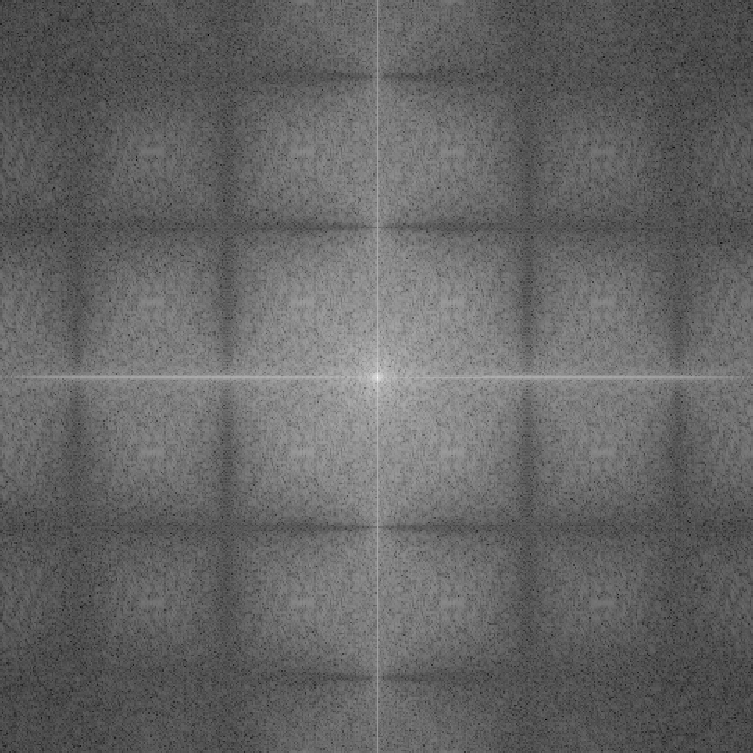
\includegraphics[width=\textwidth]{2/3_abs_fourier_log_norm_img_gaussian.png}
        \caption{Изображение $\log{(1+|\mathcal{F}\{K_\sigma*pic\}|)}$}
    \end{minipage}\hfill
    \begin{minipage}{0.49\textwidth}
        \centering 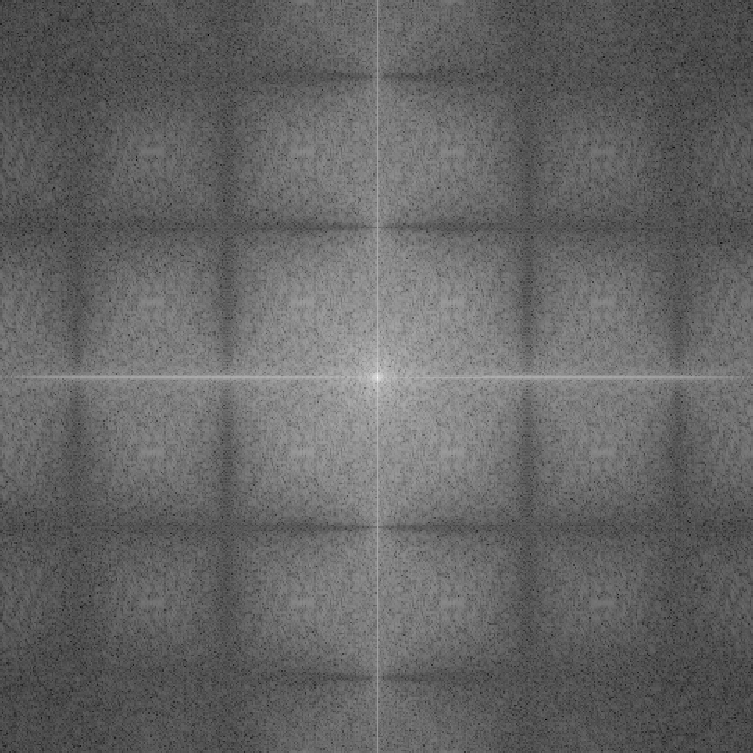
\includegraphics[width=\textwidth]{2/3_abs_fourier_log_norm_img_gaussian1.png}
        \caption{Изображение $\log{(1+|\mathcal{F}\{\mathcal{F}^{-1}\{ \mathcal{F}\{K_\sigma\}\mathcal{F}\{pic\}\}\}|)}$}
    \end{minipage}\\[1em]
\end{figure}\noindent\

Фильтрованные изображения в сравнении с исходным при выбранном $N$:

\begin{figure}[H]
    \centering
    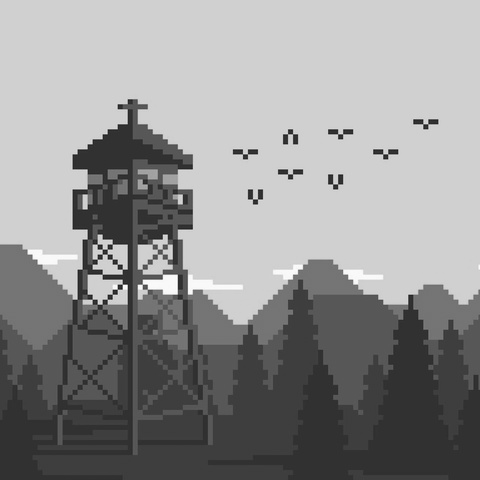
\includegraphics[width=0.51\linewidth]{2/image.png}
    \caption{Исходное изображение}
\end{figure}\

\begin{figure}[H]
    \begin{minipage}{0.49\textwidth}
        \centering 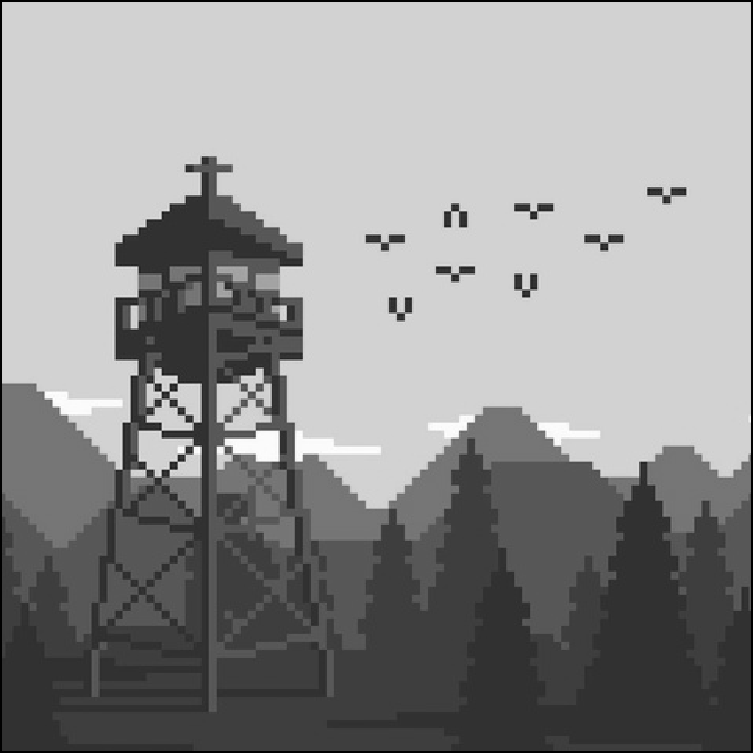
\includegraphics[width=\textwidth]{2/3_img_gaussian_by_conv2.png}
        \caption{Фильтрованное (свертка)}
    \end{minipage}\hfill
    \begin{minipage}{0.49\textwidth}
        \centering 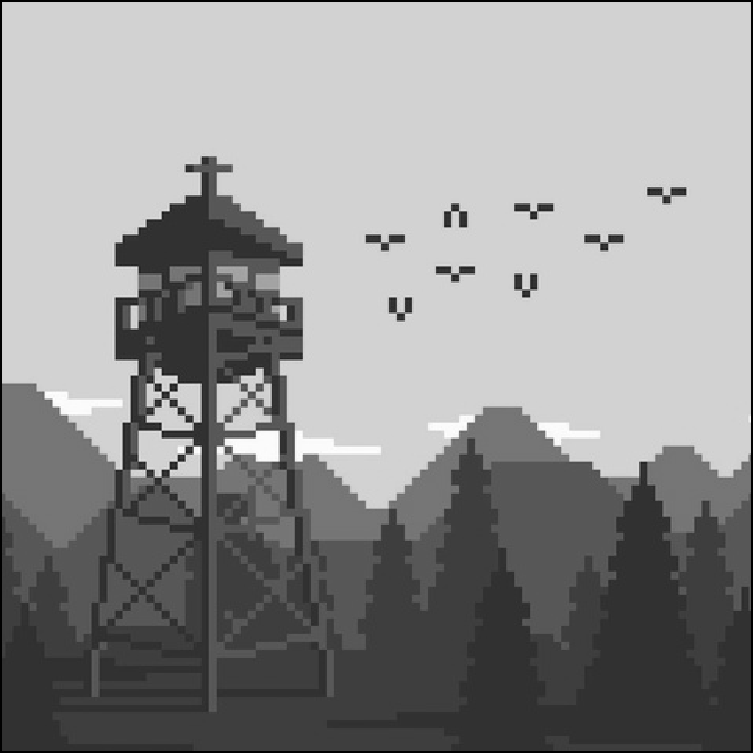
\includegraphics[width=\textwidth]{2/3_img_gaussian_by_fourier.png}
        \caption{Фильтрованное (преобразование Фурье)}
    \end{minipage}\\[1em]
\end{figure}\noindent\

При $N = 11$:

\begin{figure}[H]
    \centering
    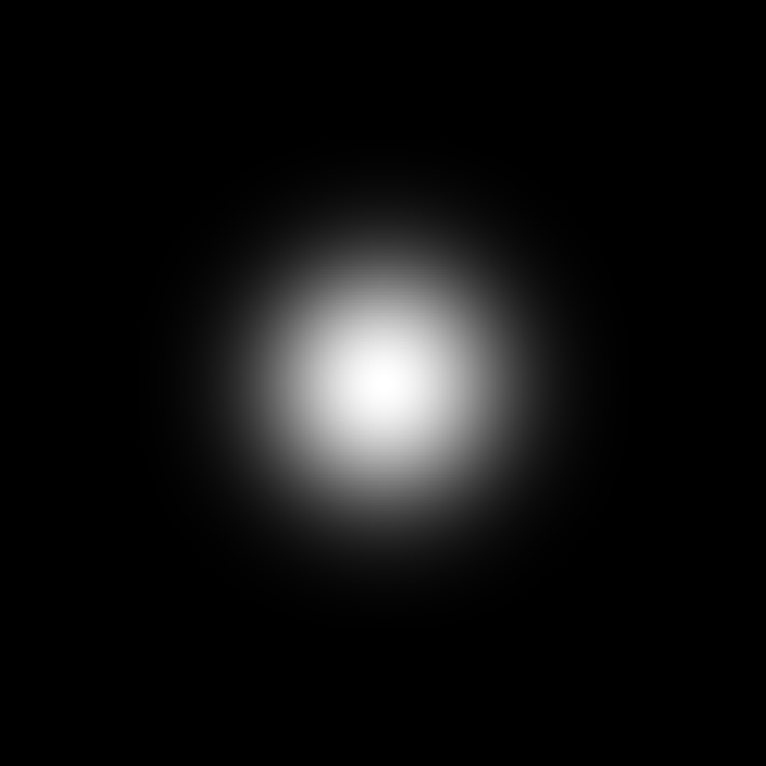
\includegraphics[width=0.51\linewidth]{2/11_abs_fourier_log_norm_gaussian.png}
    \caption{Изображение логарифма модуля образа ядра блочного размытия}
\end{figure}\

\begin{figure}[H]
    \begin{minipage}{0.49\textwidth}
        \centering 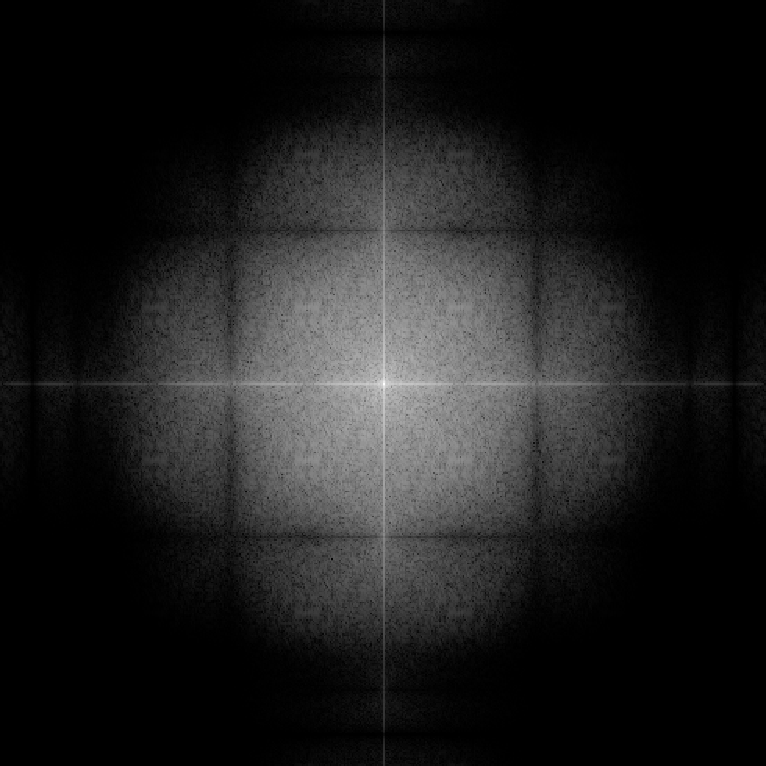
\includegraphics[width=\textwidth]{2/11_abs_fourier_log_norm_img_gaussian.png}
        \caption{Изображение $\log{(1+|\mathcal{F}\{K_\sigma*pic\}|)}$}
    \end{minipage}\hfill
    \begin{minipage}{0.49\textwidth}
        \centering 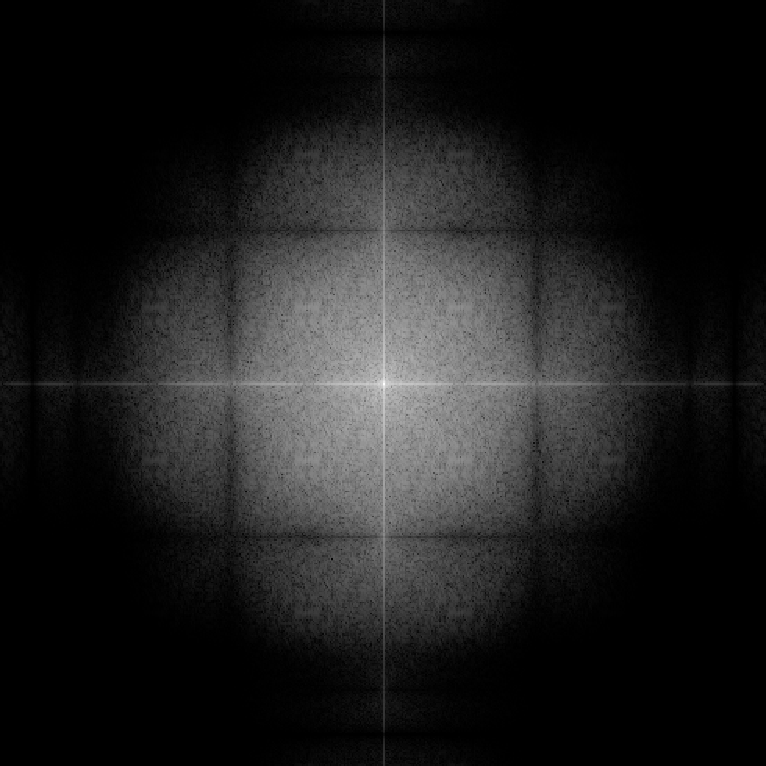
\includegraphics[width=\textwidth]{2/11_abs_fourier_log_norm_img_gaussian1.png}
        \caption{Изображение $\log{(1+|\mathcal{F}\{\mathcal{F}^{-1}\{ \mathcal{F}\{K_\sigma\}\mathcal{F}\{pic\}\}\}|)}$}
    \end{minipage}\\[1em]
\end{figure}\noindent\

Фильтрованные изображения в сравнении с исходным при выбранном $N$:

\begin{figure}[H]
    \centering
    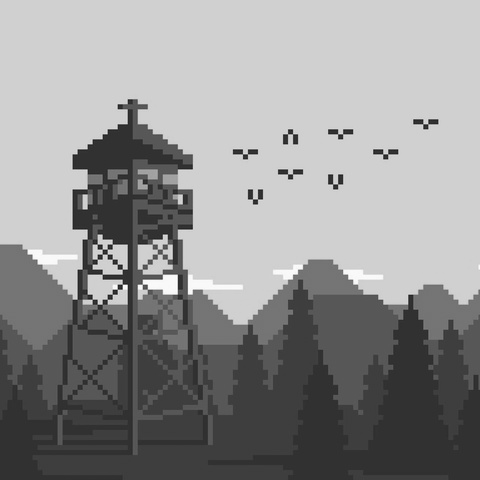
\includegraphics[width=0.51\linewidth]{2/image.png}
    \caption{Исходное изображение}
\end{figure}\

\begin{figure}[H]
    \begin{minipage}{0.49\textwidth}
        \centering 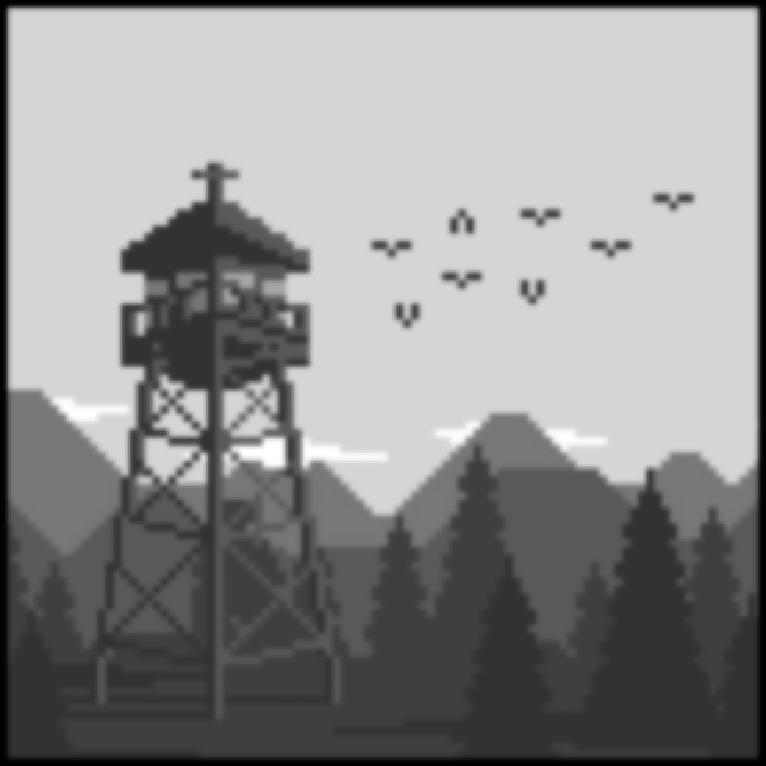
\includegraphics[width=\textwidth]{2/11_img_gaussian_by_conv2.png}
        \caption{Фильтрованное (свертка)}
    \end{minipage}\hfill
    \begin{minipage}{0.49\textwidth}
        \centering 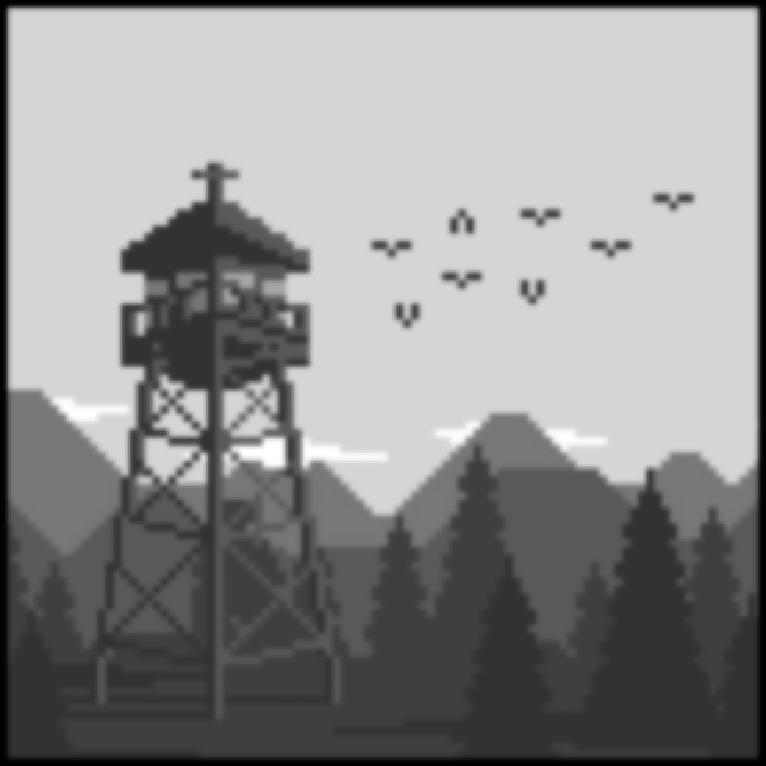
\includegraphics[width=\textwidth]{2/11_img_gaussian_by_fourier.png}
        \caption{Фильтрованное (преобразование Фурье)}
    \end{minipage}\\[1em]
\end{figure}\noindent\

При $N = 19$:

\begin{figure}[H]
    \centering
    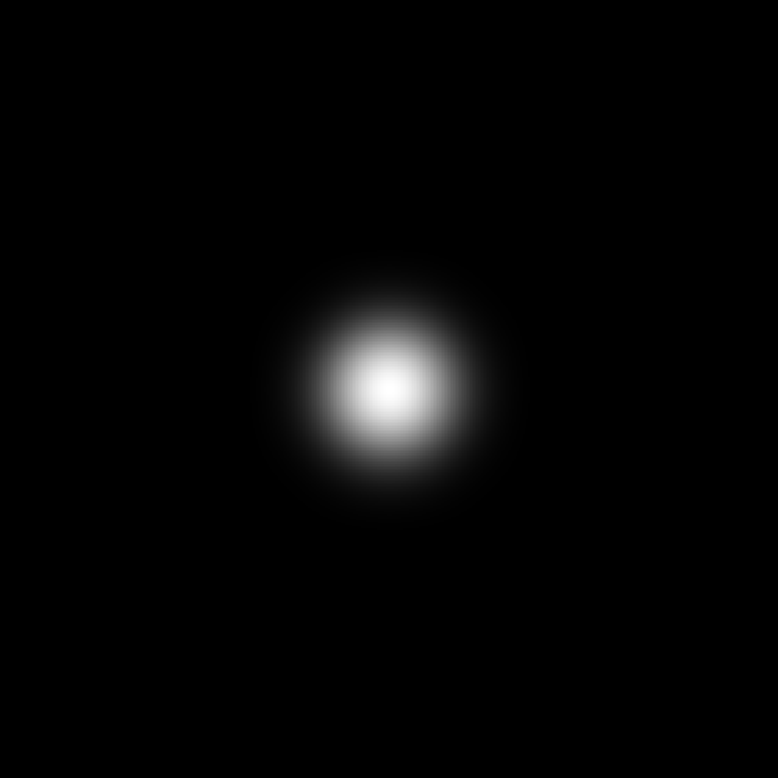
\includegraphics[width=0.51\linewidth]{2/19_abs_fourier_log_norm_gaussian.png}
    \caption{Изображение логарифма модуля образа ядра блочного размытия}
\end{figure}\

\begin{figure}[H]
    \begin{minipage}{0.49\textwidth}
        \centering 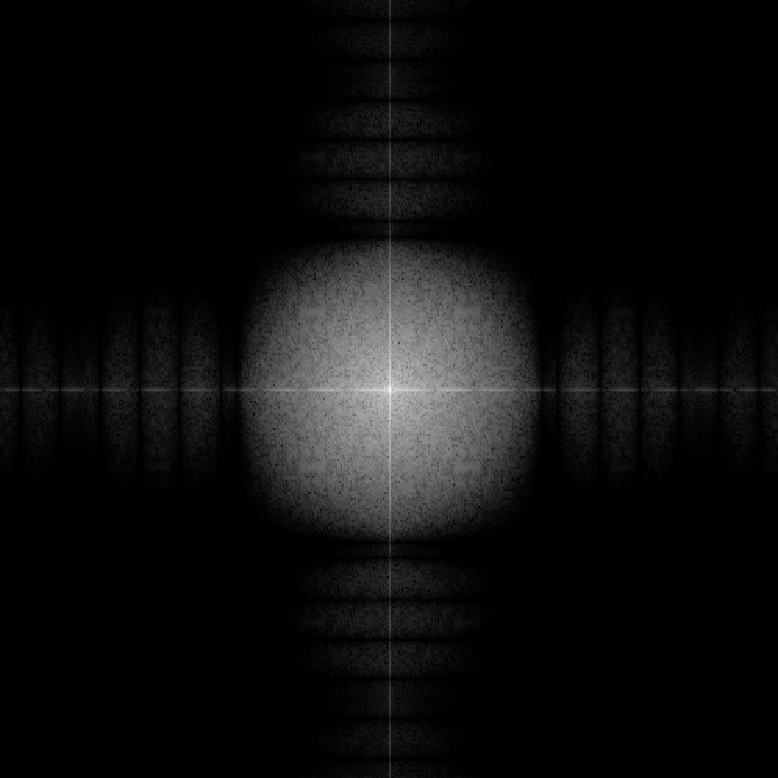
\includegraphics[width=\textwidth]{2/19_abs_fourier_log_norm_img_gaussian.png}
        \caption{Изображение $\log{(1+|\mathcal{F}\{K_\sigma*pic\}|)}$}
    \end{minipage}\hfill
    \begin{minipage}{0.49\textwidth}
        \centering 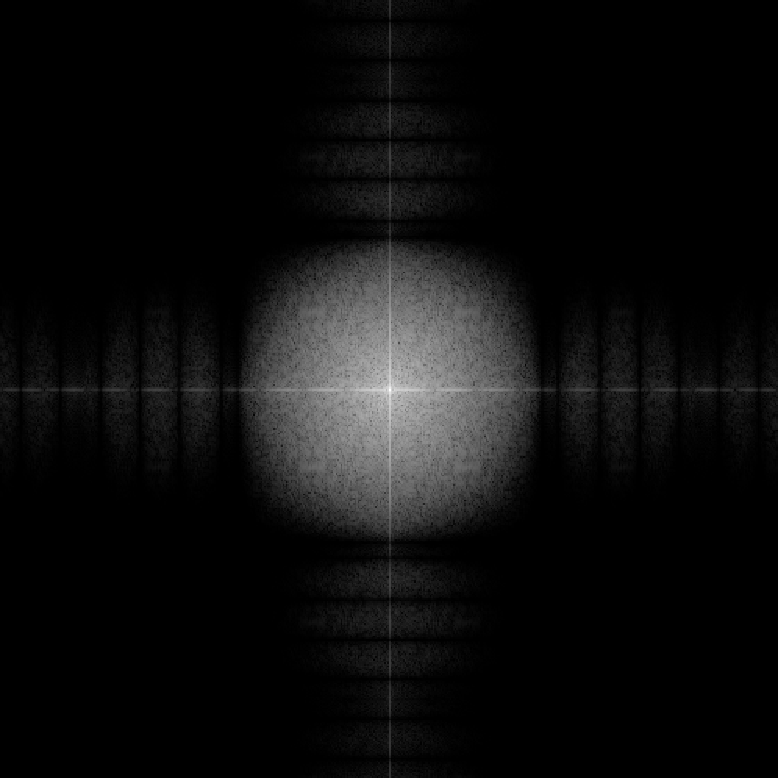
\includegraphics[width=\textwidth]{2/19_abs_fourier_log_norm_img_gaussian1.png}
        \caption{Изображение $\log{(1+|\mathcal{F}\{\mathcal{F}^{-1}\{ \mathcal{F}\{K_\sigma\}\mathcal{F}\{pic\}\}\}|)}$}
    \end{minipage}\\[1em]
\end{figure}\noindent\

Фильтрованные изображения в сравнении с исходным при выбранном $N$:

\begin{figure}[H]
    \centering
    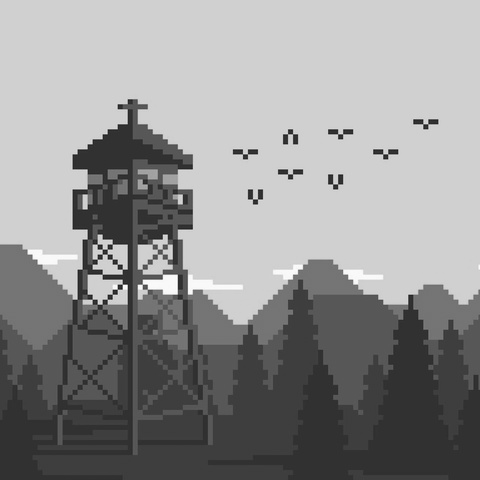
\includegraphics[width=0.51\linewidth]{2/image.png}
    \caption{Исходное изображение}
\end{figure}\

\begin{figure}[H]
    \begin{minipage}{0.49\textwidth}
        \centering 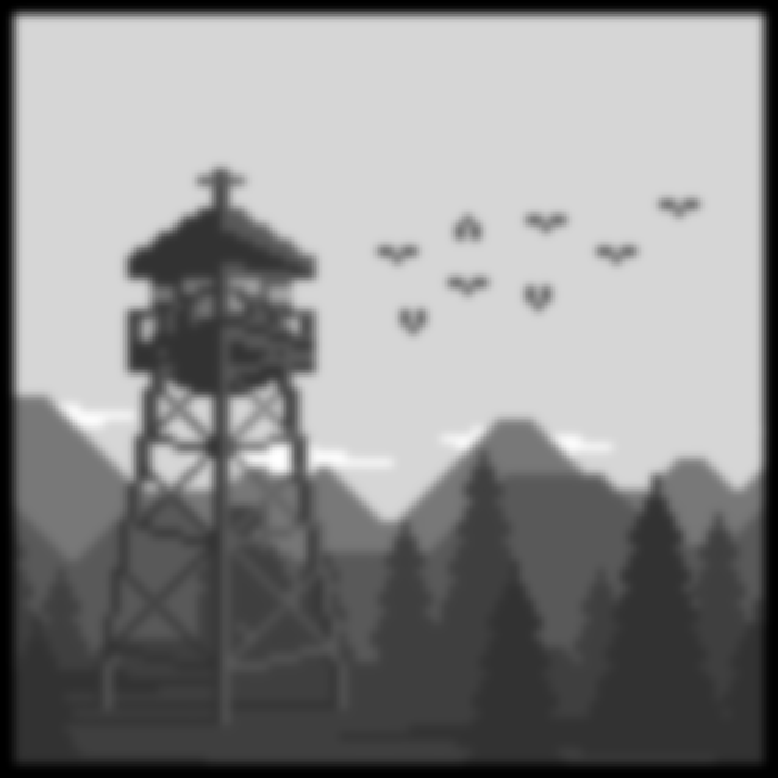
\includegraphics[width=\textwidth]{2/19_img_gaussian_by_conv2.png}
        \caption{Фильтрованное (свертка)}
    \end{minipage}\hfill
    \begin{minipage}{0.49\textwidth}
        \centering 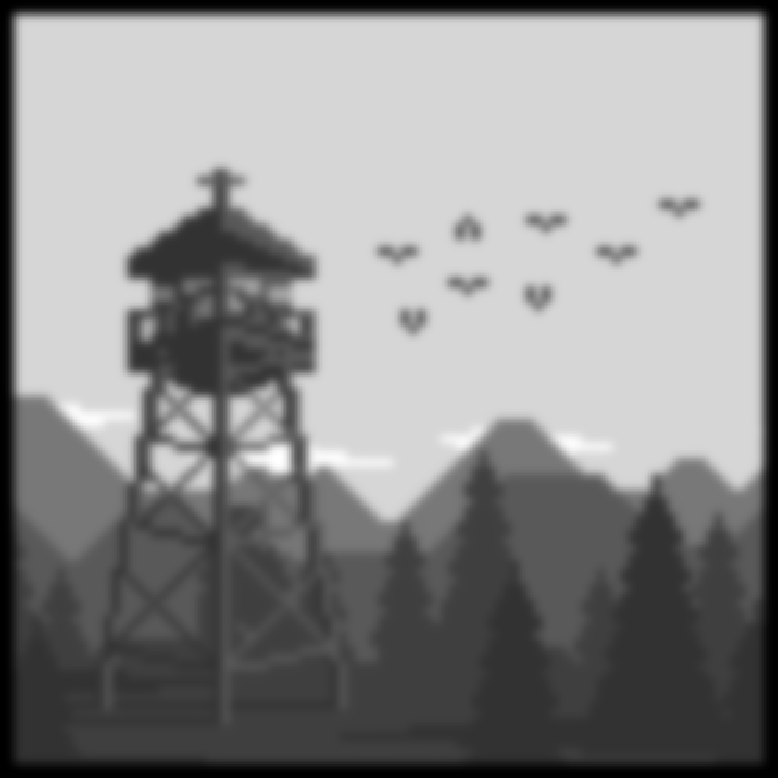
\includegraphics[width=\textwidth]{2/19_img_gaussian_by_fourier.png}
        \caption{Фильтрованное (преобразование Фурье)}
    \end{minipage}\\[1em]
\end{figure}\noindent

\subsection{Ядро блочного размытия}\ 

Вид этого ядра также зависит от $N$:

$$
A_{ij} = 1, \, i,j \in \{1, \dots, N \}, \, K_{\boxed{}} = \frac{A}{\sum_{i,j} A_{i,j}}.
$$\ 

Также как и предыдущее, свернем его с исходным изображением при разных $N$ и сравним результат последовательно сначала с исходным, а затем с обратным преобразованием Фурье от образов исходного изображения и ядра свертки. При $N = 3$:

\begin{figure}[H]
    \centering
    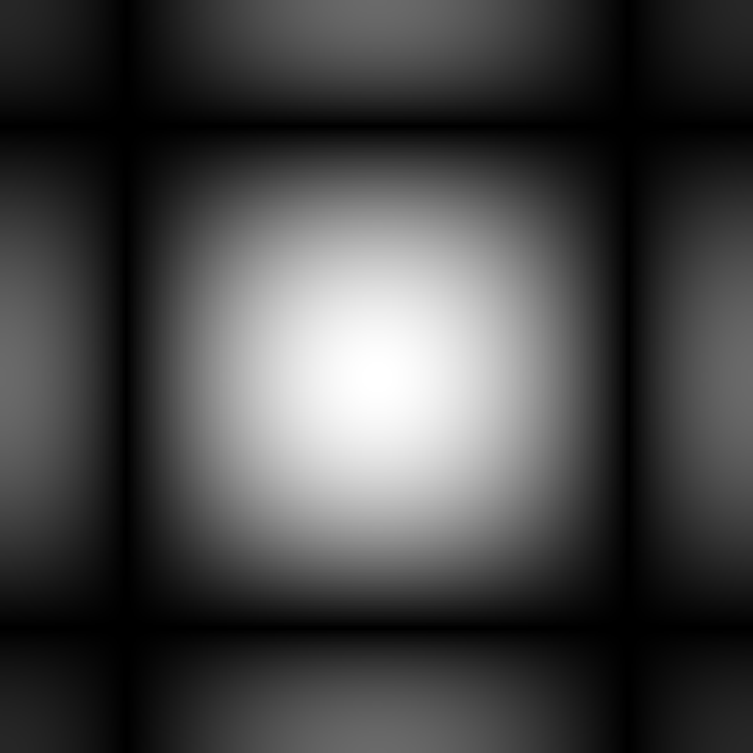
\includegraphics[width=0.51\linewidth]{2/3_abs_fourier_log_norm_block.png}
    \caption{Изображение логарифма модуля образа ядра блочного размытия}
\end{figure}\noindent

\begin{figure}[H]
    \begin{minipage}{0.49\textwidth}
        \centering 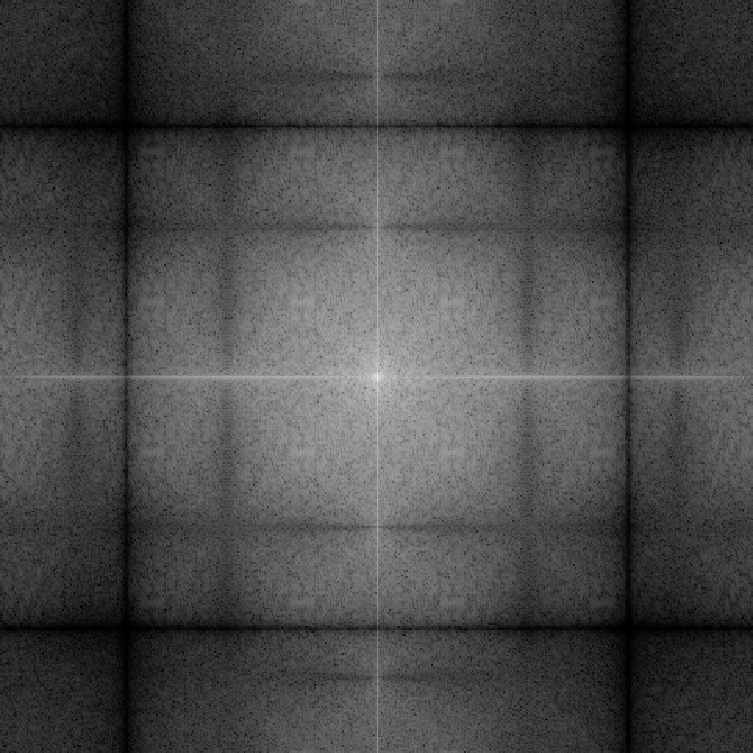
\includegraphics[width=\textwidth]{2/3_abs_fourier_log_norm_img_block.png}
        \caption{Изображение $\log{(1+|\mathcal{F}\{K_{\boxed{}}*pic\}|)}$}
    \end{minipage}\hfill
    \begin{minipage}{0.49\textwidth}
        \centering 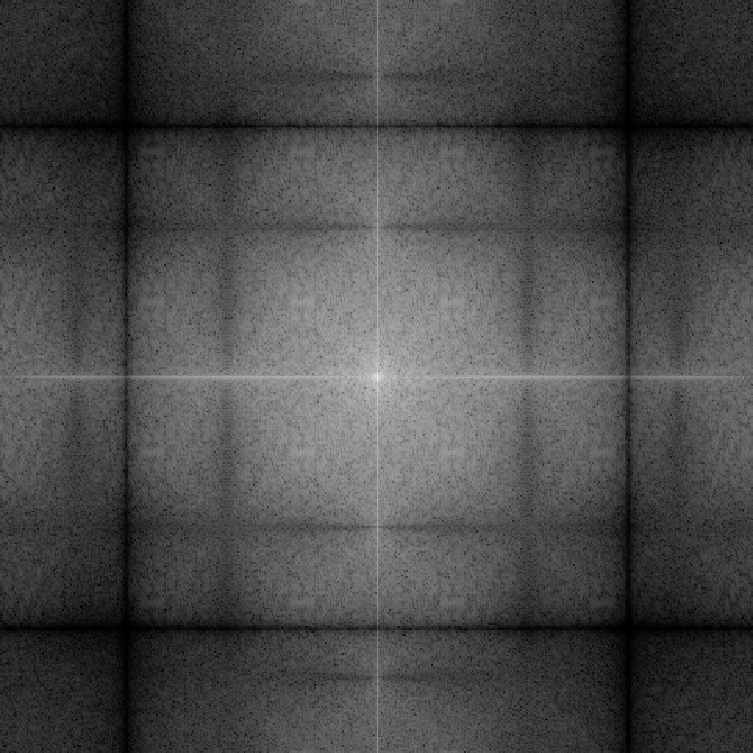
\includegraphics[width=\textwidth]{2/3_abs_fourier_log_norm_img_block1.png}
        \caption{Изображение $\log{(1+|\mathcal{F}\{\mathcal{F}^{-1}\{ \mathcal{F}\{K_{\boxed{}}\}\mathcal{F}\{pic\}\}\}|)}$}
    \end{minipage}\\[1em]
\end{figure}\noindent\

Фильтрованные изображения в сравнении с исходным при выбранном $N$:

\begin{figure}[H]
    \centering
    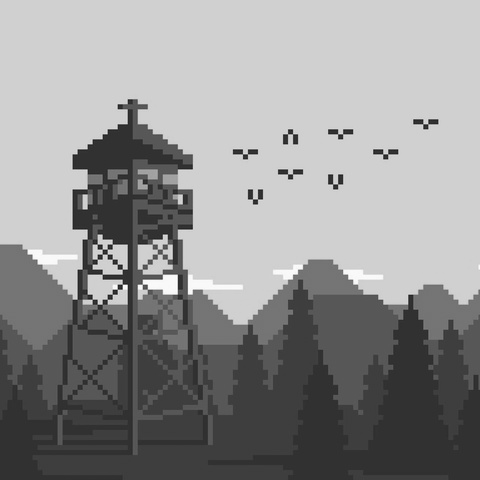
\includegraphics[width=0.51\linewidth]{2/image.png}
    \caption{Исходное изображение}
\end{figure}\

\begin{figure}[H]
    \begin{minipage}{0.49\textwidth}
        \centering 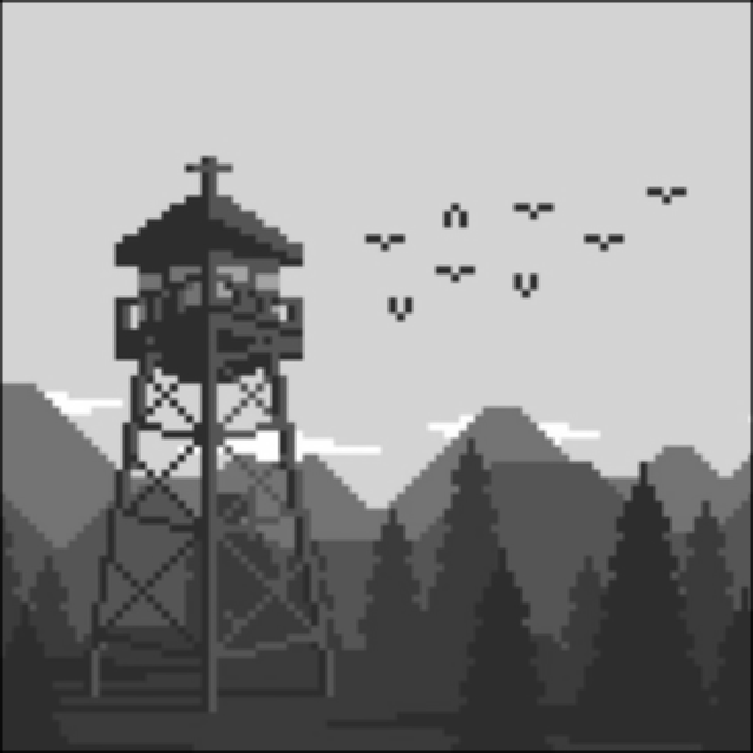
\includegraphics[width=\textwidth]{2/3_img_block_by_conv2.png}
        \caption{Фильтрованное (свертка)}
    \end{minipage}\hfill
    \begin{minipage}{0.49\textwidth}
        \centering 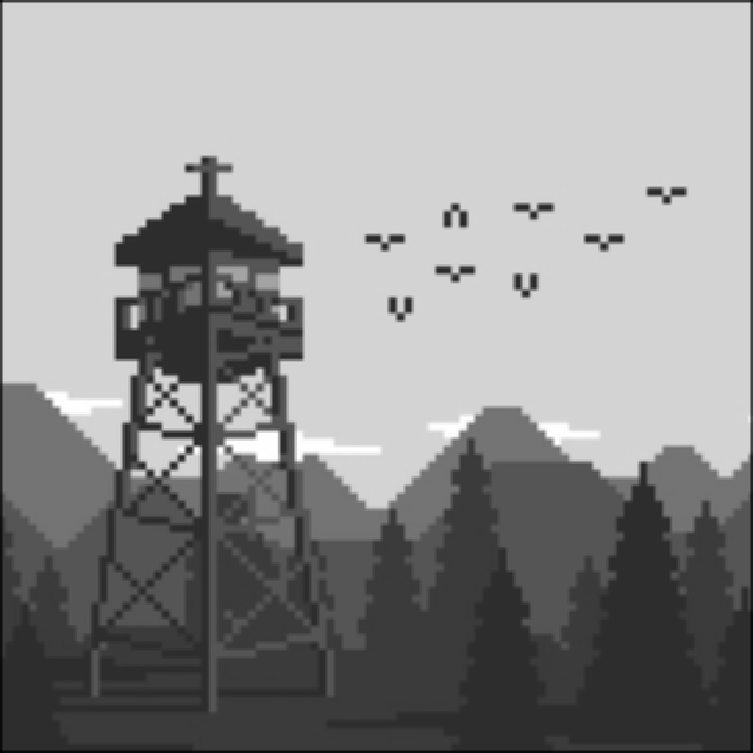
\includegraphics[width=\textwidth]{2/3_img_block_by_fourier.png}
        \caption{Фильтрованное (преобразование Фурье)}
    \end{minipage}\\[1em]
\end{figure}\noindent\

При $N = 11$:

\begin{figure}[H]
    \centering
    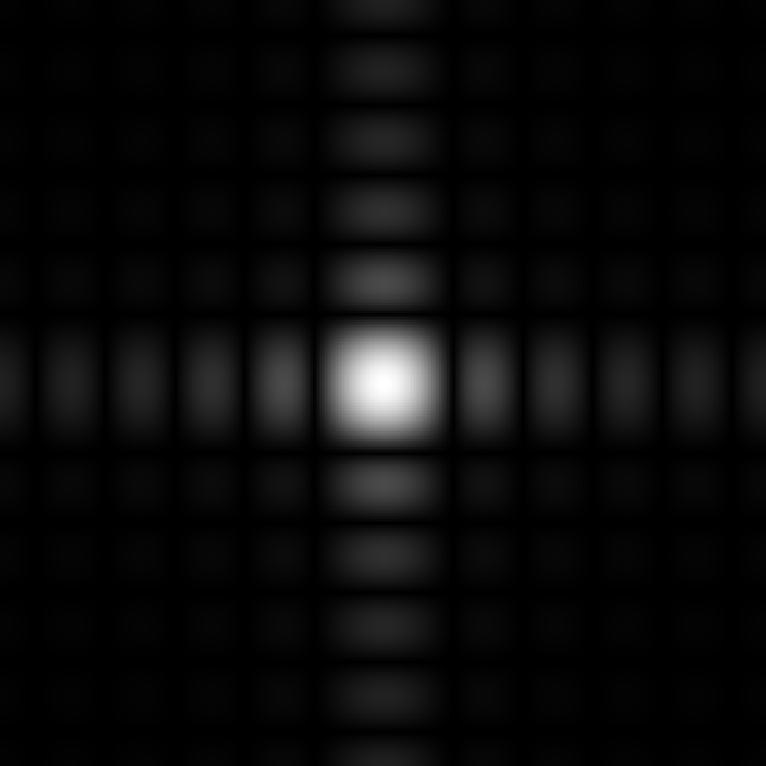
\includegraphics[width=0.51\linewidth]{2/11_abs_fourier_log_norm_block.png}
    \caption{Изображение логарифма модуля образа ядра блочного размытия}
\end{figure}\

\begin{figure}[H]
    \begin{minipage}{0.49\textwidth}
        \centering 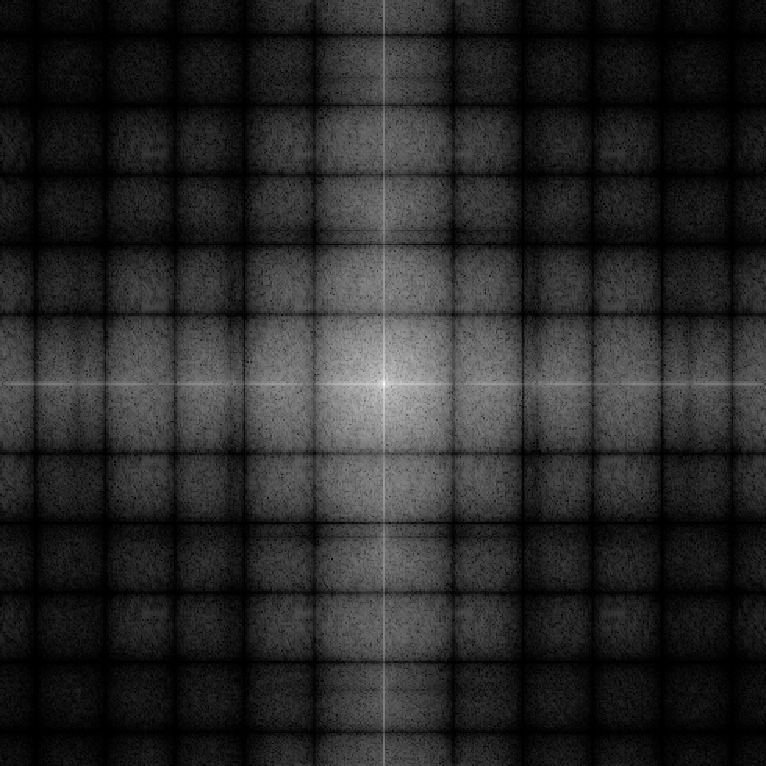
\includegraphics[width=\textwidth]{2/11_abs_fourier_log_norm_img_block.png}
        \caption{Изображение $\log{(1+|\mathcal{F}\{K_{\boxed{}}*pic\}|)}$}
    \end{minipage}\hfill
    \begin{minipage}{0.49\textwidth}
        \centering 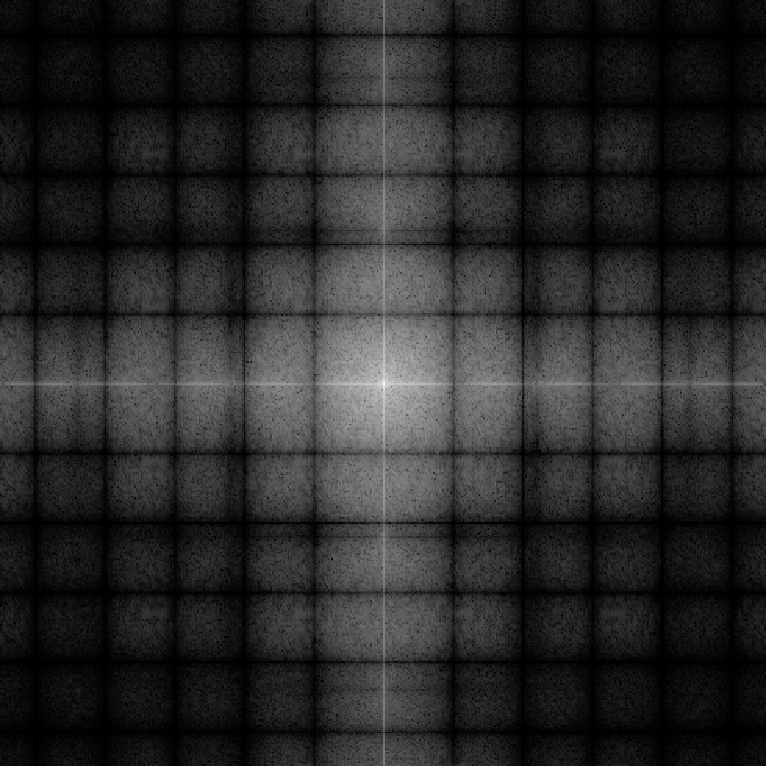
\includegraphics[width=\textwidth]{2/11_abs_fourier_log_norm_img_block1.png}
        \caption{Изображение $\log{(1+|\mathcal{F}\{\mathcal{F}^{-1}\{ \mathcal{F}\{K_{\boxed{}}\}\mathcal{F}\{pic\}\}\}|)}$}
    \end{minipage}\\[1em]
\end{figure}\noindent\

Фильтрованные изображения в сравнении с исходным при выбранном $N$:

\begin{figure}[H]
    \centering
    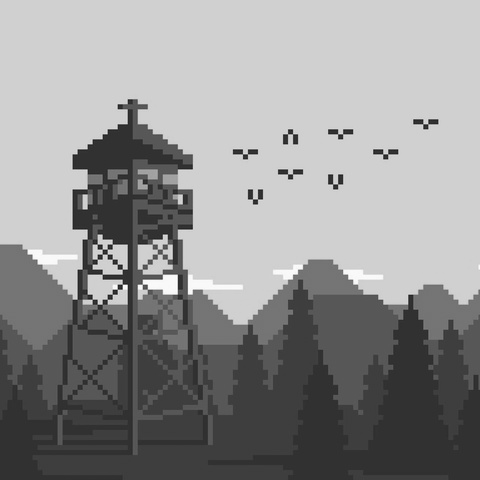
\includegraphics[width=0.51\linewidth]{2/image.png}
    \caption{Исходное изображение}
\end{figure}\

\begin{figure}[H]
    \begin{minipage}{0.49\textwidth}
        \centering 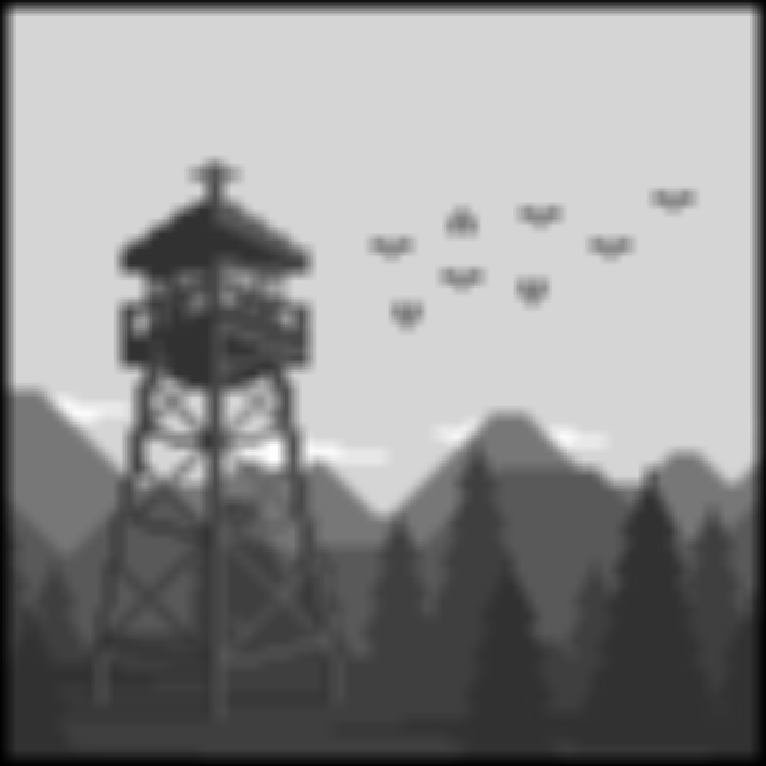
\includegraphics[width=\textwidth]{2/11_img_block_by_conv2.png}
        \caption{Фильтрованное (свертка)}
    \end{minipage}\hfill
    \begin{minipage}{0.49\textwidth}
        \centering 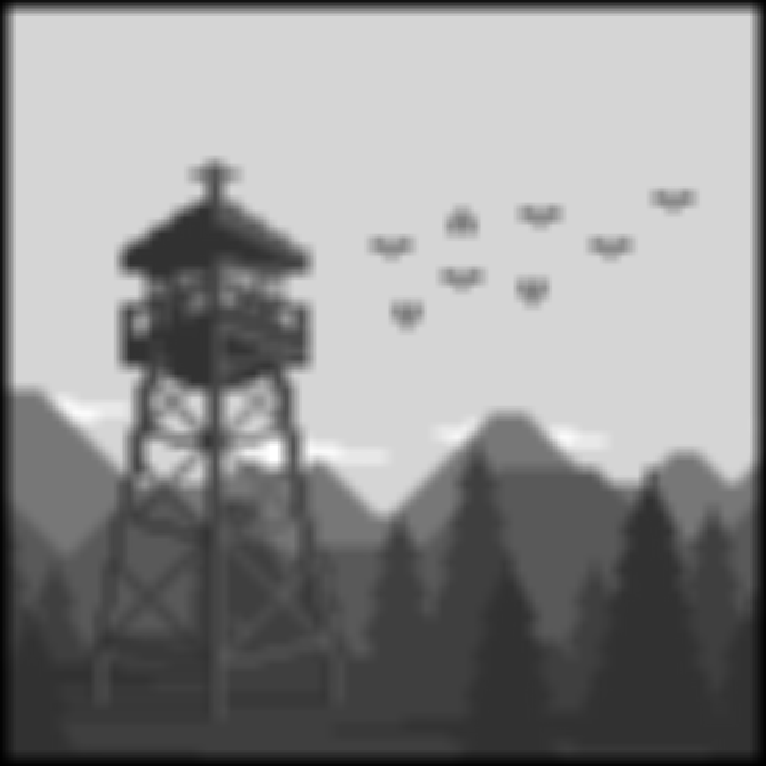
\includegraphics[width=\textwidth]{2/11_img_block_by_fourier.png}
        \caption{Фильтрованное (преобразование Фурье)}
    \end{minipage}\\[1em]
\end{figure}\noindent\

При $N = 19$:

\begin{figure}[H]
    \centering
    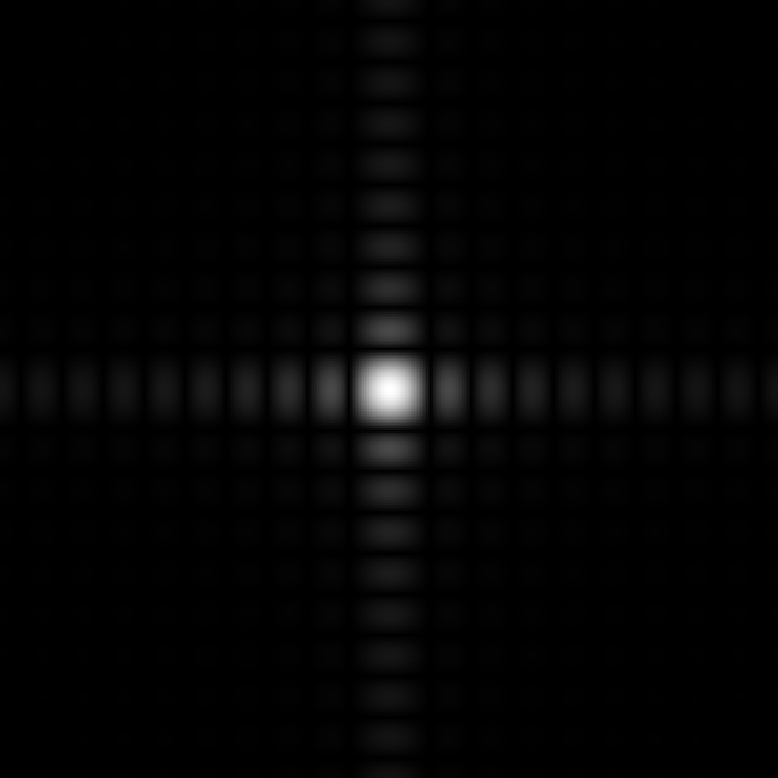
\includegraphics[width=0.51\linewidth]{2/19_abs_fourier_log_norm_block.png}
    \caption{Изображение логарифма модуля образа ядра блочного размытия}
\end{figure}\

\begin{figure}[H]
    \begin{minipage}{0.49\textwidth}
        \centering 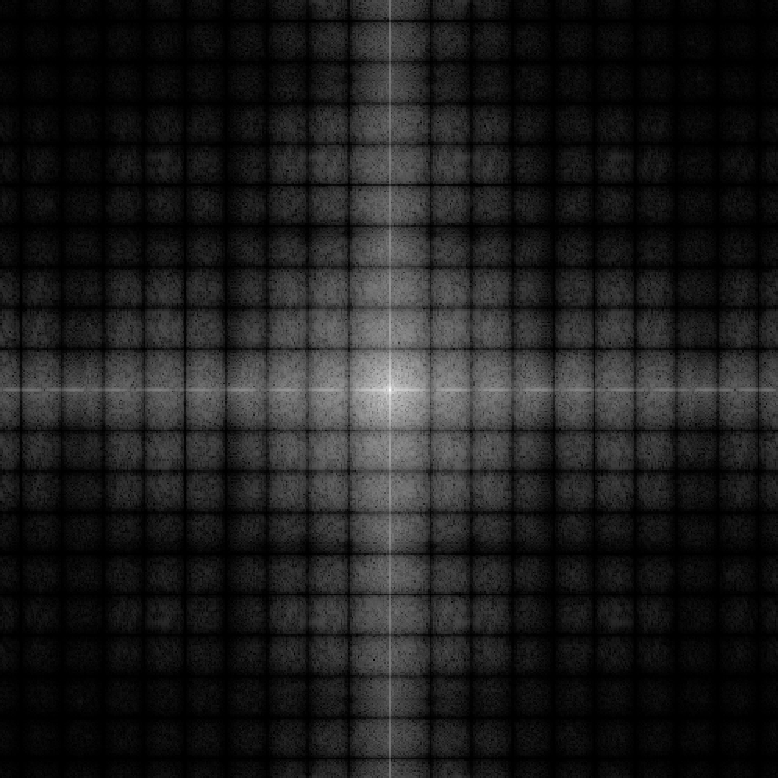
\includegraphics[width=\textwidth]{2/19_abs_fourier_log_norm_img_block.png}
        \caption{Изображение $\log{(1+|\mathcal{F}\{K_{\boxed{}}*pic\}|)}$}
    \end{minipage}\hfill
    \begin{minipage}{0.49\textwidth}
        \centering 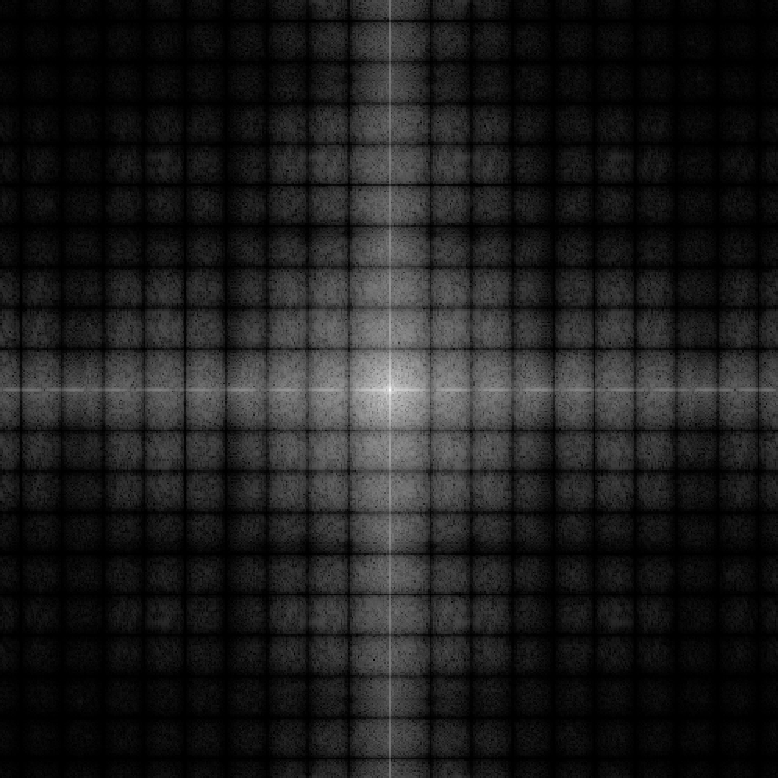
\includegraphics[width=\textwidth]{2/19_abs_fourier_log_norm_img_block1.png}
        \caption{Изображение $\log{(1+|\mathcal{F}\{\mathcal{F}^{-1}\{ \mathcal{F}\{K_{\boxed{}}\}\mathcal{F}\{pic\}\}\}|)}$}
    \end{minipage}\\[1em]
\end{figure}\noindent\

Фильтрованные изображения в сравнении с исходным при выбранном $N$:

\begin{figure}[H]
    \centering
    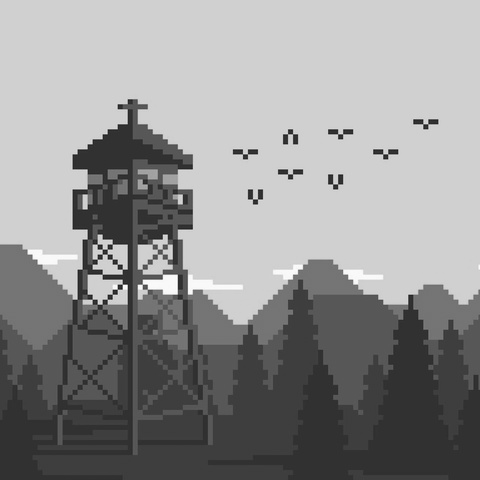
\includegraphics[width=0.51\linewidth]{2/image.png}
    \caption{Исходное изображение}
\end{figure}\

\begin{figure}[H]
    \begin{minipage}{0.49\textwidth}
        \centering 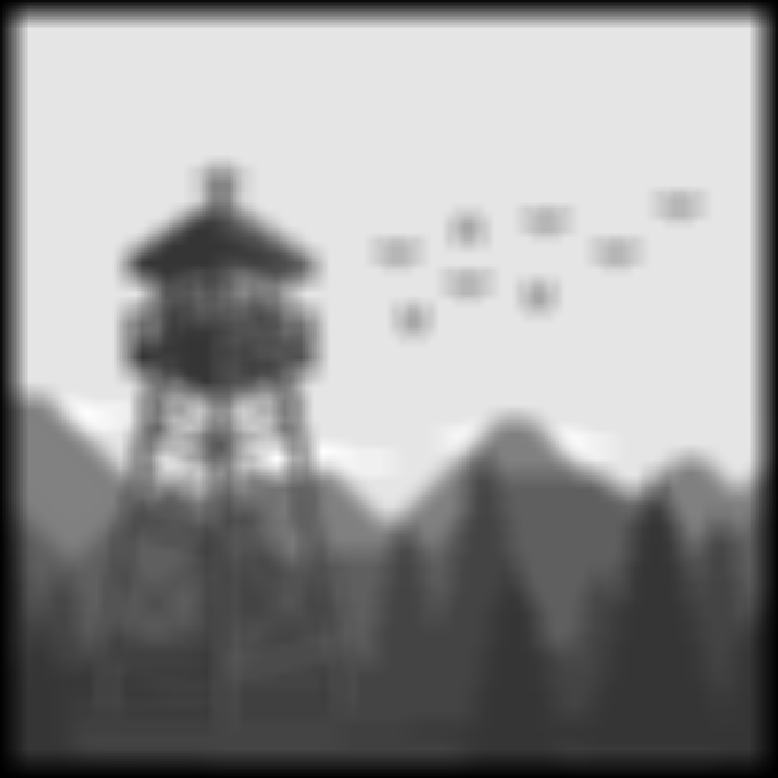
\includegraphics[width=\textwidth]{2/19_img_block_by_conv2.png}
        \caption{Фильтрованное (свертка)}
    \end{minipage}\hfill
    \begin{minipage}{0.49\textwidth}
        \centering 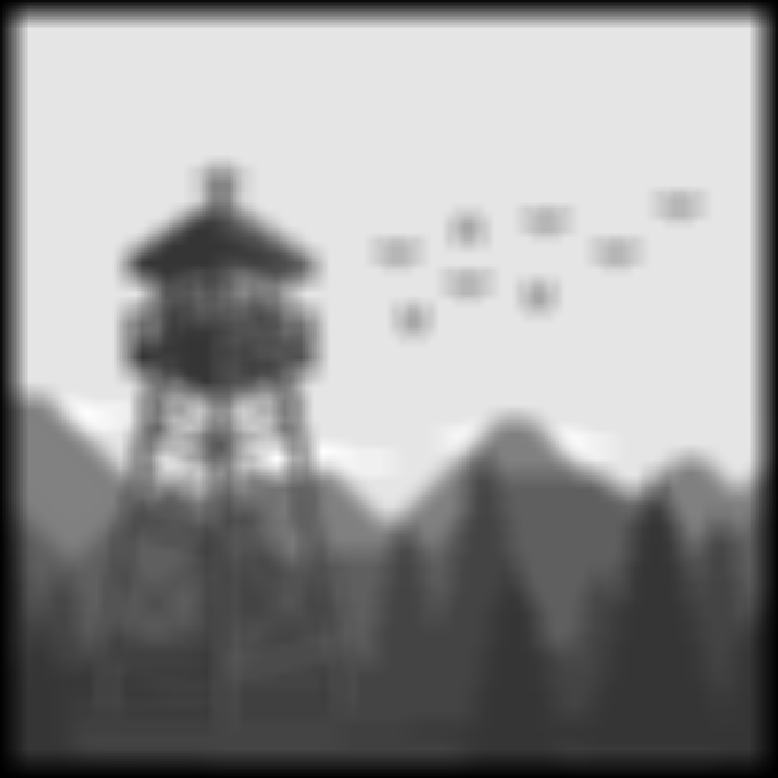
\includegraphics[width=\textwidth]{2/19_img_block_by_fourier.png}
        \caption{Фильтрованное (преобразование Фурье)}
    \end{minipage}\\[1em]
\end{figure}\noindent\

Отдельно сравним качество Гауссовского и блочного размытия при $N = 11$ и $N = 19$:

\begin{figure}[H]
    \begin{minipage}{0.49\textwidth}
        \centering 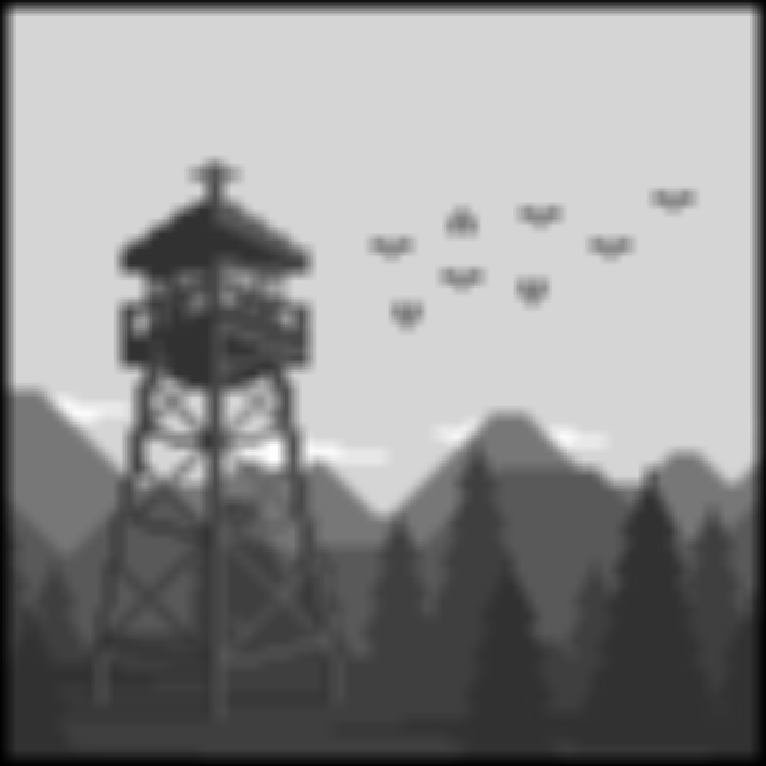
\includegraphics[width=\textwidth]{2/11_img_block_by_conv2.png}
        \caption{Размытие блочное ($N = 11$)}
    \end{minipage}\hfill
    \begin{minipage}{0.49\textwidth}
        \centering 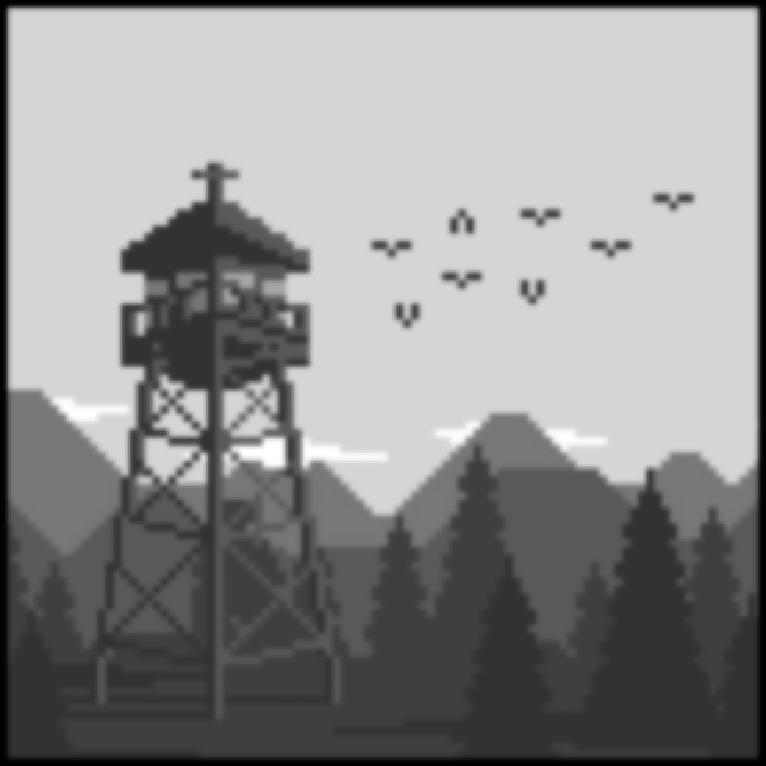
\includegraphics[width=\textwidth]{2/11_img_gaussian_by_conv2.png}
        \caption{Размытие по Гауссу ($N = 11$)}
    \end{minipage}\\[1em]
\end{figure}\noindent\

\begin{figure}[H]
    \begin{minipage}{0.49\textwidth}
        \centering 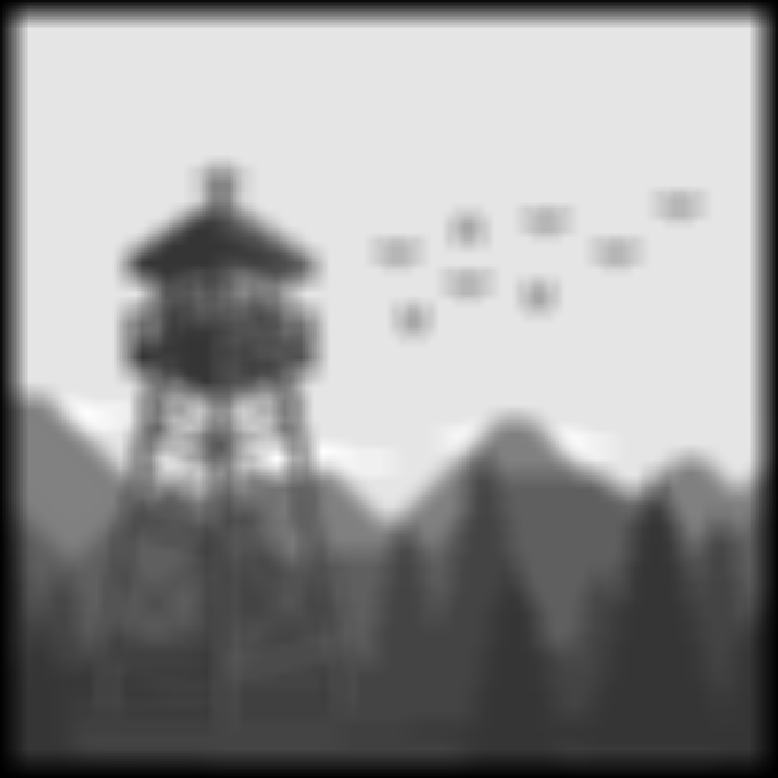
\includegraphics[width=\textwidth]{2/19_img_block_by_conv2.png}
        \caption{Размытие блочное ($N = 19$)}
    \end{minipage}\hfill
    \begin{minipage}{0.49\textwidth}
        \centering \includegraphics[width=\textwidth]{2/19_img_gaussian_by_conv2.png}
        \caption{Размытие по Гауссу ($N = 19$)}
    \end{minipage}\\[1em]
\end{figure}\noindent\

При использовании блочного размытия изображение меняется заметно сильнее при равном $N$, но складывается такое ощущение, что одновременно с резкостью картинка теряет ещё и качество (образуются блоки со средним значением цвета пикселей, и чем выше $N$, тем они более заметны), в то время как размытие по Гауссу более естественно, походит на расфокусированную фотографию.

\subsection{Ядро увеличения резкости}\ 

Это ядро выглядит следующим образом:

$$
K_* = \begin{bmatrix}
    0 & -1 & 0 \\ 
    -1 & 5 & -1 \\ 
    0 & -1 & 0
\end{bmatrix}.
$$\

Снова посмотрим на оригинальное изображение и сравним фильтрацию при помощи свертки с этим ядром и при помощи преобразования Фурье:

\begin{figure}[H]
    \centering
    \includegraphics[width=0.45\linewidth]{2/abs_fourier_log_norm_sharpen.png}
    \caption{Изображение логарифма модуля образа ядра увеличения резкости}
\end{figure}\noindent

\begin{figure}[H]
    \begin{minipage}{0.49\textwidth}
        \centering \includegraphics[width=\textwidth]{2/abs_fourier_log_norm_img_sharpen.png}
        \caption{Изображение $\log{(1+|\mathcal{F}\{K_**pic\}|)}$}
    \end{minipage}\hfill
    \begin{minipage}{0.49\textwidth}
        \centering \includegraphics[width=\textwidth]{2/abs_fourier_log_norm_img_sharpen1.png}
        \caption{Изображение $\log{(1+|\mathcal{F}\{\mathcal{F}^{-1}\{ \mathcal{F}\{K_*\}\mathcal{F}\{pic\}\}\}|)}$}
    \end{minipage}\\[1em]
\end{figure}\noindent\

Фильтрованные изображения в сравнении с исходным и друг с другом:

\begin{figure}[H]
    \centering
    \includegraphics[width=0.51\linewidth]{2/image.png}
    \caption{Исходное изображение}
\end{figure}\

\begin{figure}[H]
    \begin{minipage}{0.49\textwidth}
        \centering \includegraphics[width=\textwidth]{2/img_sharpen_by_conv2.png}
        \caption{Фильтрованное (свертка)}
    \end{minipage}
    \begin{minipage}{0.49\textwidth}
        \centering \includegraphics[width=\textwidth]{2/img_sharpen_by_fourier.png}
        \caption{Фильтрованное (преобразование Фурье)}
    \end{minipage}
\end{figure}\noindent\

\subsection{Ядро выделения краёв}\ 

Это ядро выглядит следующим образом:

$$K_\bigtriangledown
\begin{bmatrix}
    -1 & -1 & -1 \\
    -1 & 8 & -1 \\
    -1 & -1 & -1
\end{bmatrix}
$$\

Снова посмотрим на оригинальное изображение и сравним фильтрацию при помощи свертки с этим ядром и при помощи преобразования Фурье:

\begin{figure}[H]
    \centering
    \includegraphics[width=0.47\linewidth]{2/abs_fourier_log_norm_edge.png}
    \caption{Изображение логарифма модуля образа ядра выделения краев}
\end{figure}\noindent

\begin{figure}[H]
    \begin{minipage}{0.49\textwidth}
        \centering \includegraphics[width=\textwidth]{2/abs_fourier_log_norm_img_edge.png}
        \caption{Изображение $\log{(1+|\mathcal{F}\{K_**pic\}|)}$}
    \end{minipage}\hfill
    \begin{minipage}{0.49\textwidth}
        \centering \includegraphics[width=\textwidth]{2/abs_fourier_log_norm_img_edge1.png}
        \caption{Изображение $\log{(1+|\mathcal{F}\{\mathcal{F}^{-1}\{ \mathcal{F}\{K_*\}\mathcal{F}\{pic\}\}\}|)}$}
    \end{minipage}\\[1em]
\end{figure}\noindent\

Фильтрованные изображения в сравнении с исходным и друг с другом:

\begin{figure}[H]
    \centering
    \includegraphics[width=0.51\linewidth]{2/image.png}
    \caption{Исходное изображение}
\end{figure}\

\begin{figure}[H]
    \begin{minipage}{0.49\textwidth}
        \centering \includegraphics[width=\textwidth]{2/img_edge_by_conv2.png}
        \caption{Фильтрованное (свертка)}
    \end{minipage}
    \begin{minipage}{0.49\textwidth}
        \centering \includegraphics[width=\textwidth]{2/img_edge_by_fourier.png}
        \caption{Фильтрованное (преобразование Фурье)}
    \end{minipage}
\end{figure}\noindent\

\subsection{Горизонтальное ядро Скарра}\

Помимо приведенных в задании мною было выбрано горизонтальное ядро Скарра (Scharr Kernel). Оно с большой точностью подчеркивает горизонтальные изменения интенсивности. Вот его вид:

$$K_{S} =
\begin{bmatrix}
    3 & 0 & -3 \\
    10 & 0 & -10 \\
    3 & 0 & -3
\end{bmatrix}
$$\

Снова посмотрим на оригинальное изображение и сравним фильтрацию изображения при помощи свертки с этим ядром и при помощи преобразования Фурье:

\begin{figure}[H]
    \centering
    \includegraphics[width=0.47\linewidth]{2/abs_fourier_log_norm_laplacian.png}
    \caption{Изображение логарифма модуля образа горизонтального ядра Скарра}
\end{figure}\noindent

\begin{figure}[H]
    \begin{minipage}{0.49\textwidth}
        \centering \includegraphics[width=\textwidth]{2/abs_fourier_log_norm_img_laplacian.png}
        \caption{Изображение $\log{(1+|\mathcal{F}\{K_S*pic\}|)}$}
    \end{minipage}\hfill
    \begin{minipage}{0.49\textwidth}
        \centering \includegraphics[width=\textwidth]{2/abs_fourier_log_norm_img_laplacian1.png}
        \caption{Изображение $\log{(1+|\mathcal{F}\{\mathcal{F}^{-1}\{ \mathcal{F}\{K_S\}\mathcal{F}\{pic\}\}\}|)}$}
    \end{minipage}\\[1em]
\end{figure}\noindent\

Фильтрованные изображения в сравнении с исходным и друг с другом:

\begin{figure}[H]
    \centering
    \includegraphics[width=0.51\linewidth]{2/image.png}
    \caption{Исходное изображение}
\end{figure}\

\begin{figure}[H]
    \begin{minipage}{0.49\textwidth}
        \centering \includegraphics[width=\textwidth]{2/img_laplacian_by_conv2.png}
        \caption{Фильтрованное (свертка)}
    \end{minipage}
    \begin{minipage}{0.49\textwidth}
        \centering \includegraphics[width=\textwidth]{2/img_laplacian_by_fourier.png}
        \caption{Фильтрованное (преобразование Фурье)}
    \end{minipage}
\end{figure}\noindent\

\subsection{Выводы}\ 

Изображения, полученные с помощью свёртки и с помощью Фурье-преобразования, не отличаются, что подтверждает равенство $f * g = \mathcal{F}^{-1}\{\mathcal{F}\{f\}\mathcal{F}\{g\}\}$. Также для выделения краёв изображения уменьшалась амплитуда образа в центре изображения, а для наложения размытия (и сохранения основных частей изображения) подавлялось изображение логарифма модуля образа ближе к краям, центр наоборот оставался неизменным. Это подчеркивает сходство с фильтрацией в случае одномерного преобразования -- основная часть изображения (раньше -- сигнала) сосредоточена в центре (в окрестности нуля) изображения логарифма модуля образа (в одномерном случае -- графика образа), а мелкие детали и помехи -- по краям.

\section{Вывод по работе}\

В результате проведенной работы я осознал, как сглаживать изображения с периодичностью (подобно сигналу с гармоническими помехами в случае одномерного преобразования, однако теперь соответствующие помехам пики видны не ``сбоку'', а ``сверху'', и представляют собой светлые точки на графике), а также освоил ядра свёртки, несколько похожие на двумерный аналог фильтра.

\newpage

\section{Приложение А. Код для выполнения заданий}

\subsection*{Листинг 1. Код для выполнения задания 1}

\begin{lstlisting}[caption={Код для построения графиков для задания 1}, language=matlab]
image = double(imread("3.png"))./255;
fourier = fftshift(fft2(image));

abs_fourier = abs(fourier);
angle_fourier = angle(fourier);

abs_fourier_log = log(abs_fourier + 1);

abs_fourier_log_norm = abs_fourier_log./max(abs_fourier_log(:), [], 'all');

imwrite(abs_fourier_log_norm, "im3_fourier.png")
recovered_log = double(imread("im3_fourier_recovered.png"))./255;


recovered_abs_log = recovered_log .* max(abs_fourier_log(:), [], 'all');
recovered_abs = exp(recovered_abs_log) - 1;
recovered_fourier = recovered_abs .* exp(1i * angle_fourier);
recovered_image = real(ifft2(ifftshift(recovered_fourier)));
imwrite(recovered_image, "im3_recovered.png");
\end{lstlisting}

\subsection*{Листинг 2. Код для выполнения задания 2}

\begin{lstlisting}[caption={Код для построения графиков для задания 2}, language=matlab]
close all;
image = imread("firewatch480.jpg");
image_gray = im2gray(image);
imwrite(image_gray, strcat('2', filesep, 'image.png'));
global h;
global w;
global N;
[h, w] = size(image_gray);

% Ядро размытия по Гауссу
N = 3;
sigma = (N - 1) / 6;
A = zeros(N, N);
center = (N + 1) / 2;
for i = 1:N
    for j = 1:N
        A(i,j) = exp(-((i - center)^2 + (j - center)^2) / (2 * sigma^2));
    end
end
K_gaussian = A / sum(A, 'all');
[k_gaussian, l_gaussian] = size(K_gaussian); 

% Ядро блочного размытия
K_block = ones(N);
K_block = K_block / sum(K_block, 'all');
[k_block, l_block] = size(K_block); 

% Ядро увеличения резкости
K_sharpen = [0 -1 0; -1 5 -1; 0 -1 0];
[k_sharpen, l_sharpen] = size(K_sharpen); 

% Ядро выделения краев
K_edge = [-1 -1 -1; -1 8 -1; -1 -1 -1];
[k_edge, l_edge] = size(K_edge); 

% Ядро Скарра (раньше тут был Laplacian of Gaussian, поэтому переменная названа так)
K_laplacian = [3 0 -3; 10 0 -10; 3 0 -3];
[k_laplacian, l_laplacian] = size(K_laplacian); 

img_gaussian = conv2(image_gray, K_gaussian);
img_block = conv2(image_gray, K_block);
img_sharpen = conv2(image_gray, K_sharpen);
img_edge = conv2(image_gray, K_edge);
img_laplacian = conv2(image_gray, K_laplacian);

h_g = figure;
imshow(img_gaussian, [],"Border","tight");
h_b = figure;
imshow(img_block, [],"Border","tight");
imwrite(img_sharpen, strcat('2', filesep, 'img_sharpen_by_conv2.png'));
imwrite(img_edge, strcat('2', filesep, 'img_edge_by_conv2.png'));
imwrite(img_laplacian, strcat('2', filesep, 'img_laplacian_by_conv2.png'));
saveas(h_g, strcat('2', filesep, num2str(N), '_img_gaussian_by_conv2', '.png'), 'png')
saveas(h_b, strcat('2', filesep, num2str(N), '_img_block_by_conv2', '.png'), 'png')

% Логарифмы модулей обазов

function abs_fourier_log_norm = ln_mod_fourier(data, k, l, arg_name)
    global h;
    global w;
    global N;
    fourier = fftshift(fft2(data, h+k-1,w+l-1));
    abs_fourier = abs(fourier);
    abs_fourier_log = log(abs_fourier + 1);
    abs_fourier_log_norm = abs_fourier_log./max(abs_fourier_log(:), [], 'all');
    h1 = figure;
    imshow(abs_fourier_log_norm, [],"Border","tight");
    if (k == 3)
        saveas(h1, strcat('2', filesep, 'abs_fourier_log_norm_', arg_name, '.png'), 'png');
    else
        saveas(h1, strcat('2', filesep, num2str(k), '_abs_fourier_log_norm_', arg_name, '.png'), 'png');
    end
end
ln_mod_fourier(image_gray, 3, 3, 'image');
ln_mod_fourier(K_gaussian, N, N, 'gaussian');
ln_mod_fourier(K_block, N, N, 'block');
ln_mod_fourier(K_sharpen, 3, 3, 'sharpen');
ln_mod_fourier(K_edge, 3, 3, 'edge');
ln_mod_fourier(K_laplacian, 3, 3, 'laplacian');

% Фурье-образы

fourier_image = fft2(image_gray,h+k_sharpen-1,w+l_sharpen-1);
fourier_image_n = fft2(image_gray,h+k_gaussian-1,w+l_gaussian-1);

fourier_gaussian = fft2(K_gaussian,h+k_gaussian-1,w+l_gaussian-1);
fourier_block = fft2(K_block,h+k_block-1,w+l_block-1);
fourier_sharpen = fft2(K_sharpen,h+k_sharpen-1,w+l_sharpen-1);
fourier_edge = fft2(K_edge,h+k_edge-1,w+l_edge-1);
fourier_laplacian = fft2(K_laplacian,h+k_laplacian-1,w+l_laplacian-1);

% Умножение образа изображения на образы ядер

img_gaussian_fourier = fourier_image_n .* fourier_gaussian;
img_block_fourier = fourier_image_n .* fourier_block;
img_sharpen_fourier = fourier_image .* fourier_sharpen;
img_edge_fourier = fourier_image .* fourier_edge;
img_laplacian_fourier = fourier_image .* fourier_laplacian;

% Обратные преобразования Фурье от полученных произведений

img_gaussian1 = real(ifft2(img_gaussian_fourier));
img_block1 = ifft2(img_block_fourier);
img_sharpen1 = real(ifft2(img_sharpen_fourier));
img_edge1 = ifft2(img_edge_fourier);
img_laplacian1 = ifft2(img_laplacian_fourier);

% Сохранение логарифмов модулей Фурье-образов получившихся изображений (сначала conv2, затем фурье)

ln_mod_fourier(img_gaussian, N, N, 'img_gaussian');
ln_mod_fourier(img_block, N, N, 'img_block');
ln_mod_fourier(img_sharpen, 3, 3, 'img_sharpen');
ln_mod_fourier(img_edge, 3, 3, 'img_edge');
ln_mod_fourier(img_laplacian, 3, 3, 'img_laplacian');

ln_mod_fourier(img_gaussian1, N, N, 'img_gaussian1');
ln_mod_fourier(img_block1, N, N, 'img_block1');
ln_mod_fourier(img_sharpen1, 3, 3, 'img_sharpen1');
ln_mod_fourier(img_edge1, 3, 3, 'img_edge1');
ln_mod_fourier(img_laplacian1, 3, 3, 'img_laplacian1');

% Отображение полученных изображений

h_g1 = figure;
imshow(img_gaussian1, [],"Border","tight");
h_b1 = figure;
imshow(img_block1, [],"Border","tight");
imwrite(img_sharpen1, strcat('2', filesep, 'img_sharpen_by_fourier.png'))
imwrite(img_edge1, strcat('2', filesep, 'img_edge_by_fourier.png'))
imwrite(img_laplacian1, strcat('2', filesep, 'img_laplacian_by_fourier.png'))
saveas(h_g1, strcat('2', filesep, num2str(N), '_img_gaussian_by_fourier', '.png'), 'png')
saveas(h_b1, strcat('2', filesep, num2str(N), '_img_block_by_fourier', '.png'), 'png')
% close all;
\end{lstlisting}
\end{document}
